\documentclass[a4paper,12pt,twoside]{memoir}

% Castellano
\usepackage[spanish,es-tabla]{babel}
\selectlanguage{spanish}
\usepackage[utf8]{inputenc}
\usepackage[T1]{fontenc}
\usepackage{lmodern} % Scalable font
\usepackage{microtype}
\usepackage{placeins}

\RequirePackage{booktabs}
\RequirePackage[table]{xcolor}
\RequirePackage{xtab}
\RequirePackage{multirow}

% Links
\PassOptionsToPackage{hyphens}{url}\usepackage[colorlinks]{hyperref}
\hypersetup{
	allcolors = {red}
}

% Ecuaciones
\usepackage{amsmath}

% Rutas de fichero / paquete
\newcommand{\ruta}[1]{{\sffamily #1}}

% Párrafos
\nonzeroparskip

% Huérfanas y viudas
\widowpenalty100000
\clubpenalty100000

\let\tmp\oddsidemargin
\let\oddsidemargin\evensidemargin
\let\evensidemargin\tmp
\reversemarginpar

% Imágenes

% Comando para insertar una imagen en un lugar concreto.
% Los parámetros son:
% 1 --> Ruta absoluta/relativa de la figura
% 2 --> Texto a pie de figura
% 3 --> Tamaño en tanto por uno relativo al ancho de página
\usepackage{graphicx}

\newcommand{\imagen}[3]{
	\begin{figure}[!h]
		\centering
		\includegraphics[width=#3\textwidth]{#1}
		\caption{#2}\label{fig:#1}
	\end{figure}
	\FloatBarrier
}







\graphicspath{ {./img/} }

% Capítulos
\chapterstyle{bianchi}
\newcommand{\capitulo}[2]{
	\setcounter{chapter}{#1}
	\setcounter{section}{0}
	\setcounter{figure}{0}
	\setcounter{table}{0}
	\chapter*{#2}
	\addcontentsline{toc}{chapter}{#2}
	\markboth{#2}{#2}
}

% Apéndices
\renewcommand{\appendixname}{Apéndice}
\renewcommand*\cftappendixname{\appendixname}

\newcommand{\apendice}[1]{
	%\renewcommand{\thechapter}{A}
	\chapter{#1}
}

\renewcommand*\cftappendixname{\appendixname\ }

% Formato de portada

\makeatletter
\usepackage{xcolor}
\newcommand{\tutor}[1]{\def\@tutor{#1}}
\newcommand{\tutorb}[1]{\def\@tutorb{#1}}

\newcommand{\course}[1]{\def\@course{#1}}
\definecolor{cpardoBox}{HTML}{E6E6FF}
\def\maketitle{
  \null
  \thispagestyle{empty}
  % Cabecera ----------------
\begin{center}
  \noindent
\includegraphics[width=\textwidth]{cabeceraSalud}\vspace{1.5cm}%
\end{center}
  
  % Título proyecto y escudo salud ----------------
  \begin{center}
    \begin{minipage}[c][1.5cm][c]{.20\textwidth}
        
\includegraphics[width=\textwidth]{escudoSalud.pdf}
    \end{minipage}
  \end{center}
  
  \begin{center}
    \colorbox{cpardoBox}{%
        \begin{minipage}{.8\textwidth}
          \vspace{.5cm}\Large
          \begin{center}
          \textbf{TFG del Grado en Ingeniería de la Salud}\vspace{.6cm}\\
          \textbf{\LARGE\@title{}}
          \end{center}
          \vspace{.2cm}
        \end{minipage}
    }%
  \end{center}
  
    % Datos de alumno, curso y tutores ------------------
  \begin{center}%
  {%
    \noindent\LARGE
    Presentado por \@author{}\\ 
    en Universidad de Burgos\\
    \vspace{0.5cm}
    \noindent\Large
    \@date{}\\
    \vspace{0.5cm}
    %Tutor: \@tutor{}\\ % comenta el que no corresponda
    Tutores: \@tutor{} -- \@tutorb{}\\
  }%
  \end{center}%
  \null
  \cleardoublepage
  }
\makeatother

\newcommand{\nombre}{Lucía Segura Benito}
\newcommand{\nombreTutor}{Daniel Sarabia Ortiz} 
\newcommand{\nombreTutorb}{Alejandro Merino Gómez} 
\newcommand{\dni}{71830574X} 

% Datos de portada
\title{Modelado determinista de epidemias}
\author{\nombre}
\tutor{\nombreTutor}
\tutorb{\nombreTutorb}
\date{\today}


\begin{document}

\maketitle


\newpage\null\thispagestyle{empty}\newpage

%%%%%%%%%%%%%%%%%%%%%%%%%%%%%%%%%%%%%%%%%%%%%%%%%%%%%%%%%%%%%%%%%%%%%%%%%%%%%%%%%%%%%%%%
\thispagestyle{empty}


\noindent
\includegraphics[width=\textwidth]{cabeceraSalud}\vspace{1cm}

\noindent D. \nombreTutor, profesor del departamento de departamento, área de área.

\noindent Expone:

\noindent Que el alumno D. \nombre, con DNI \dni, ha realizado el Trabajo final de Grado en Ingeniería de la Salud titulado 'Modelado determinista de epidemias'. 

\noindent Y que dicho trabajo ha sido realizado por el alumno bajo la dirección del que suscribe, en virtud de lo cual se autoriza su presentación y defensa.

\begin{center} %\large
En Burgos, {\large \today}
\end{center}

\vfill\vfill\vfill

% Author and supervisor
\begin{minipage}{0.45\textwidth}
\begin{flushleft} %\large
Vº. Bº. del Tutor:\\[2cm]
D. \nombreTutor
\end{flushleft}
\end{minipage}
\hfill
\begin{minipage}{0.45\textwidth}
\begin{flushleft} %\large
Vº. Bº. del Tutor:\\[2cm]
D. \nombreTutorb
\end{flushleft}
\end{minipage}
\hfill

\vfill

% para casos con solo un tutor comentar lo anterior
% y descomentar lo siguiente
%Vº. Bº. del Tutor:\\[2cm]
%D. nombre tutor


\newpage\null\thispagestyle{empty}\newpage




\frontmatter

% Abstract en castellano
\renewcommand*\abstractname{Resumen}
\begin{abstract}
En este primer apartado se hace una \textbf{breve} presentación del tema que se aborda en el proyecto.
\end{abstract}

\renewcommand*\abstractname{Descriptores}
\begin{abstract}
Palabras separadas por comas que identifiquen el contenido del proyecto Ej: servidor web, buscador de vuelos, android \ldots
\end{abstract}

\clearpage

% Abstract en inglés
\renewcommand*\abstractname{Abstract}
\begin{abstract}
A \textbf{brief} presentation of the topic addressed in the project.
\end{abstract}

\renewcommand*\abstractname{Keywords}
\begin{abstract}
keywords separated by commas.
\end{abstract}

\clearpage

% Indices
\tableofcontents

\clearpage

\listoffigures

\clearpage

\listoftables
\clearpage


\mainmatter
\capitulo{1}{Introducción}
Las enfermedades infecciosas han acompañado al ser humano desde sus orígenes, generando crisis sanitarias de gran impacto a lo largo de la historia. Epidemias como la peste negrea, la gripe española o la pandemia de COVID-19, han puesto a prueba a los sistemas de salud pública y han motivado al desarrollo de modelos matemáticos capaces de predecir su evolución y apoyar a la toma de decisiones sanitarias. La modelización epidemiológica es una herramienta clave para comprender la dinámica de transmisión de enfermedades infecciosas, estimar la magnitud de los brotes y evaluar la eficacia de intervenciones como la vacunación, el confinamiento o el distanciamiento social.


Entre los modelos existentes, los modelos deterministas han demostrado ser especialmente útiles por su simplicidad y capacidad para captar la dinámica general de una epidemia. En este tipo de modelos, la población se divide en compartimentos, y se describe el paso de individuos entre estos grupos mediante ecuaciones diferenciales ordinarias. Según el número de compartimentos y de relaciones entre ellos, surgen diferentes modelos: SI, SIS, SIR, SEIR, entre otros. Permiten obtener indicadores clave como el número reproductivo básico, la duración estimada de la epidemia o el pico de contagios.


En este proyecto se propone el estudio, simulación y análisis de varios de estos modelos epidemiológicos deterministas utilizando las herramientas proporcionadas por \texttt{MATLAB} y \texttt{Simulink}. Estas plataformas permiten implementar visualmente los sistemas dinámicos y modificar sus parámetros, lo que es ideal para simular diferentes escenarios epidemiológicos y observar su evolución bajo distintas condiciones iniciales. Además, \texttt{Simulink} ofrece herramientas para el desarrollo de interfaces gráficas \texttt{(App Designer)}, lo que va a facilitar la visualización de los resultados y la comprensión del modelo por parte de usuarios no especializados.


El trabajo no solo tiene como finalidad construir e implementar modelos epidemiológicos con \texttt{Simulink}, sino que también analiza la influencia de los parámetros clave en el comportamiento del sistema, explorar enfermedades con datos reales y estudiar la posibilidad de aplicar técnicas de ingeniería de control para modificar la evolución del brote. El objetivo es tratar a la epidemia como un sistema dinámico susceptible de ser controlado, en el que intervenciones externas pueden actuar como entradas reguladoras del sistema.


Por tanto, este proyecto se sitúa en la intersección de la ingeniería, la matemática aplicada y la epidemiología, con un enfoque práctico orientado a la simulación, análisis y control de epidemias mediante herramientas modernas de modelado. El proyecto pretende no solo aportar una visión técnica del problema, sino también desarrollar habilidades transversales y proponer una aproximación ingenieril a fenómenos con un fuerte impacto en la sociedad.

\capitulo{2}{Objetivos}

Antes de abordar el desarrollo tanto teórico como práctico del trabajo, es fundamental establecer de forma clara los objetivos que guiarán las etapas del proyecto. Dado el carácter técnico y aplicado del estudio, se han dividido los objetivos en tres categorías. La clasificación va a permitir no solo estructurar el alcance del proyecto desde el punto de vista académico y técnico, sino que también va a reflejar el crecimiento personal y profesional que se espera alcanzar con la realización del trabajo.

\section{Objetivo general}

El objetivo principal de este trabajo es el análisis, diseño e implementación de modelos epidemiológicos deterministas mediante herramientas de simulación tanto en \texttt{MATLAB} como \texttt{Simulink}, con el propósito de estudiar la propagación de enfermedades infecciosas, evaluar estrategias de control y mejorar la comprensión del comportamiento dinámico de una epidemia.

Para ello, se utilizarán tanto parámetros hipotéticos como datos reales extraídos de enfermedades conocidas, con el fin de seleccionar el modelo más adecuado para cada caso y simular su evolución. Como parte importante del proyecto, se desarrollará una aplicación interactiva para facilitar la visualización y el análisis de los resultados obtenidos a partir de los modelos simulados.

\section{Objetivos específicos}

\begin{itemize}
  \item Implementar y comparar diferentes modelos compartimentales (SI, SIS, SIR, SEIR, además de variantes con vacunación) en \texttt{Simulink}, incluyendo sus sistemas de ecuaciones diferenciales.
  \item Analizar el significado de los diferentes parámetros de los modelos (beta, gamma, \(R_0\)…) y estudiar cómo afectan a la evolución temporal de la enfermedad en los diferentes modelos.
  \item Simular diferentes escenarios utilizando parámetros hipotéticos y reales, evaluando la capacidad predictiva del modelo.
  \item Identificar enfermedades reales que puedan ajustarse adecuadamente a cada uno de los modelos epidemiológicos estudiados, recopilando sus datos históricos y simulando su comportamiento en \texttt{Simulink} con los parámetros correspondientes.
  \item Estudiar e incorporar al modelo epidemiológico un compartimento asociado a la vacunación, analizando su efecto sobre la evolución de la epidemia y las condiciones necesarias para lograr la inmunidad colectiva.
  \item Estudiar el efecto de modificar parámetros clave para observar posibles estrategias de control y su impacto sobre el comportamiento de la epidemia.
  \item Explorar la aplicación de técnicas de ingeniería de control que permitan influir activamente sobre la evolución de la epidemia.
  \item Diseñar y desarrollar una aplicación interactiva en \texttt{App Designer} que permita al usuario introducir parámetros, visualizar en tiempo real los resultados de la simulación y analizar gráficamente la evolución del sistema.
\end{itemize}

\section{Objetivos personales}

\begin{itemize}
  \item Profundizar en el conocimiento y aplicación práctica de modelos matemáticos en el ámbito de la ingeniería biomédica y la epidemiología, desarrollando la capacidad de traducir fenómenos reales en representaciones matemáticas comprensibles.
  \item Mejorar las habilidades técnicas en \texttt{MATLAB} y \texttt{Simulink}, especialmente en el diseño de modelos dinámicos, simulación de sistemas y creación de aplicaciones interactivas mediante \texttt{App Designer}.
  \item Familiarizarse con el tratamiento, análisis e interpretación de datos reales asociados a enfermedades infecciosas, y aprender a integrarlos en modelos para ajustar sus parámetros y predecir su evolución.
  \item Desarrollar habilidades en visualización de datos y comunicación de resultados científicos a través de herramientas gráficas, mejorando la capacidad de transmitir información técnica de forma accesible.
  \item Aprender a utilizar \texttt{LaTeX} como herramienta profesional para la redacción de documentos técnicos y científicos, adquiriendo autonomía en la generación de textos estructurados, con fórmulas, referencias y formato académico.
\end{itemize}


\capitulo{3}{Conceptos teóricos}
\setcounter{secnumdepth}{3}

\section{Epidemia, pandemia y epidemiología}
En este trabajo, aunque el enfoque principal es el modelado de epidemias, se utilizarán los términos \textit{epidemia} y \textit{pandemia} de manera indistinta, dado que los modelos deterministas que se aplican no distinguen explícitamente entre ambos conceptos. Estos modelos se limitan a simular la dinámica de transmisión de una enfermedad en una población, sin considerar directamente la escala geográfica o el alcance global del brote.
No obstante, es importante señalar que, aunque estos modelos  pueden aplicarse tanto a epidemias como a pandemias, los términos no deben considerarse sinónimos, ya que su diferenciación radica en el contexto y la magnitud del fenómeno. Además, se analizarán situaciones reales que incluyen casos de ambos tipos, aprovechando la versatilidad de los modelos utilizados.

A continuación se definen ambos términos.

\subsection{Epidemia}
Una epidemia es la aparición de una enfermedad en una comunidad, zona o país durante un periodo de tiempo determinado, que afecta de forma simultánea y constante, a un número elevado de personas. En la figura se ve como afecta solo a un país  \ref{fig:epidemia}\footnote{Obtenido de \cite{bbc_ebola_2014}}. Las causas pueden ser diversas e incluyen agentes infecciosos como virus, bacterias, parásitos u hongos, así como factores ambientales y sociales que favorecen la transmisión de la enfermedad. Se considera epidemia cuando cualquier enfermedad infecciosa se descontrola temporalmente y afecta a una proporción significativa de la población.

\begin{figure}[H]
    \centering
    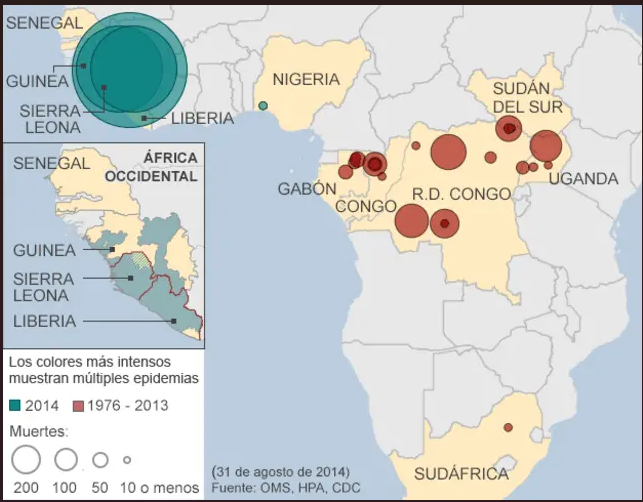
\includegraphics[width=0.7\textwidth]{img/epidemia.png}
    \caption{Ejemplo de epidemia, Ébola.}
    \label{fig:epidemia}
\end{figure}


Cabe destacar que no todas las epidemias son provocadas por enfermedades contagiosas. Aunque muchas se deben a infecciones que se transmiten entre personas, también pueden originarse por factores como el comportamiento humano, el entorno, vectores (como mosquitos) o enfermedades zoonóticas transmitidas por animales. Incluso enfermedades no transmisibles, como la obesidad o la diabetes, pueden alcanzar niveles epidémicos debido a cambios en los estilos de vida.


\subsection{Pandemia}
Una pandemia es una epidemia que se ha propagado a nivel mundial, afectando a un gran número de personas en varios países y continentes. Se caracteriza por la transmisión sostenida de persona a persona y genera un impacto significativo en la salud pública global, en la economía y la estructura social \cite{dias2024towards}. En la figura \ref{fig:pandemia}\footnote{Obtenido de \cite{isglobal_coronavirus_orden}} se puede observar como una pandemia afecta a novel global

\begin{figure}[H]
    \centering
    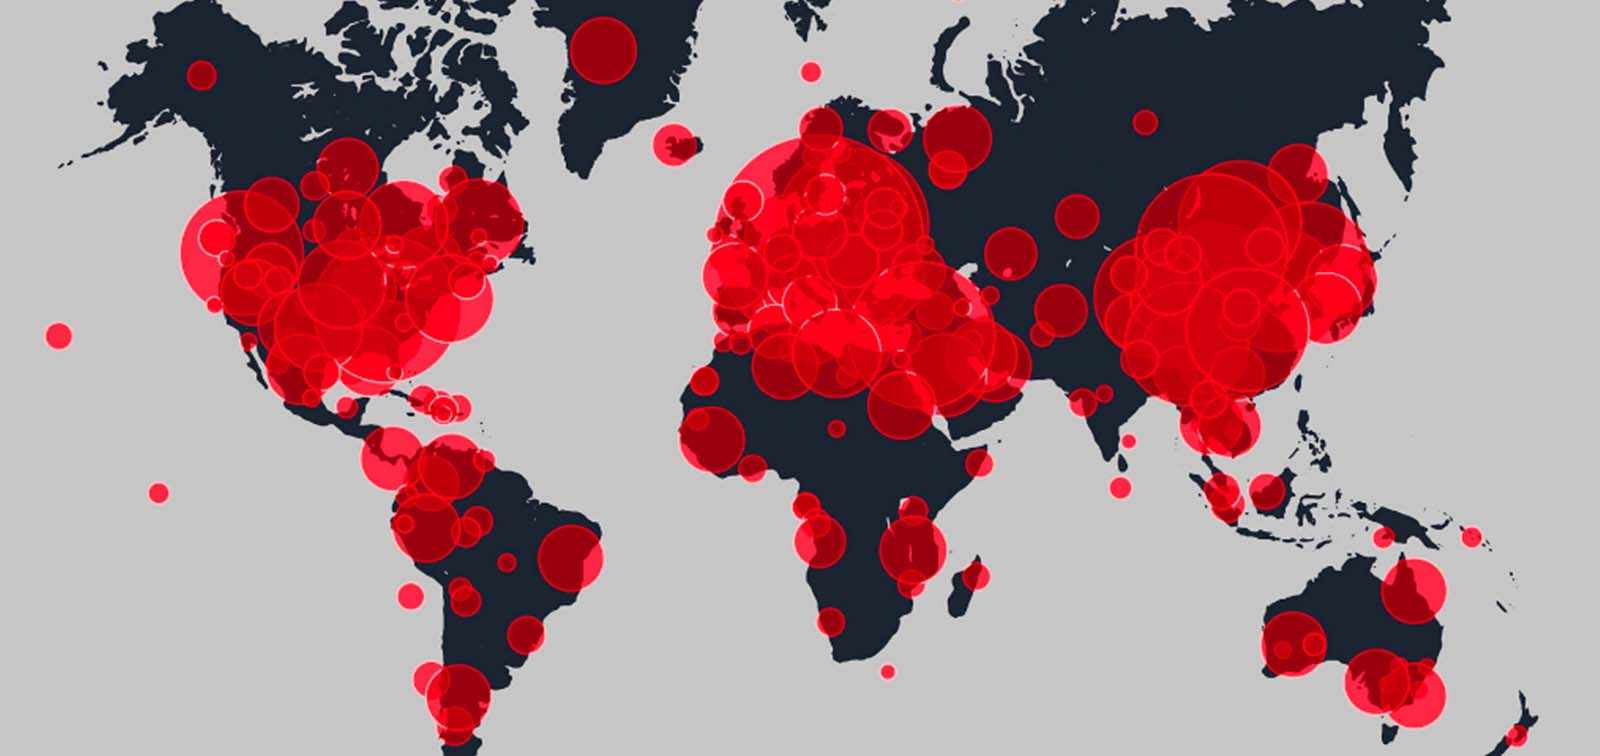
\includegraphics[width=0.7\textwidth]{img/pandemia.jpg}
    \caption{Ejemplo de pandemia, COVID-19.}
    \label{fig:pandemia}
    \vspace{0.5cm} % Ajusta el espacio vertical entre la imagen y el texto
\end{figure}

\subsection{Grupos vulnerables ante las epidemias}
Las epidemias afectan de manera desigual factores sociales, económicos y biológicos. Según \cite{nasution2021poblaciones} entre los más vulnerables se encuentran :
\begin{itemize}
  \item Personas mayores de 60 años.
  \item Personas con inmunodeficiencia.
  \item Mujeres embarazadas.
   \item Personas con obesidad.
   \item Personas con enfermedades crónicas.
   \item Grupos socioeconómicos desfavorecidos. 
\end{itemize}

\subsection{Gestión, control y prevención de epidemias}
La gestión de una epidemia requiere de diversas etapas y estrategias. La detección temprana y la vigilancia epidemiológica son fundamentales para identificar brotes y evitar su propagación. Las evaluaciones de riesgo y vulnerabilidad permiten determinar las áreas y poblaciones más afectadas. La preparación incluye la planificación de recursos, la formación del personal y la implementación de sistemas de alerta temprana.

Entre las estrategias preventivas y de control se encuentran la vacunación, el tratamiento y la mejora de las condiciones de saneamiento e higiene. La respuesta eficaz a una epidemia exige la coordinación entre distintos gobiernos, organizaciones internacionales y comunidades locales. Para erradicar la enfermedad, pueden llevarse a cabo campañas masivas de vacunación y otras intervenciones a largo plazo. Un enfoque holístico \cite{tsagkarliotis2023holistic}, que integre factores médicos, sociales, económicos, psicológicos y ambientales, resulta clave para mejorar la prevención y respuesta ante epidemias mediante la aplicación de prácticas innovadoras y enfoques interdisciplinarios. 

Los tratamientos varían según el patógeno. Entre las principales medidas de prevención y control que propone \cite{ministeriosanidad2021} se incluyen:
\begin{itemize}
  \item \textbf{Vacunación}, como herramienta fundamental en la prevención de enfermedades transmisibles.
  \item \textbf{Distanciamiento social y cuarentena}, para limitar el contacto entre personas y reducir la transmisión.
  \item \textbf{Higiene y saneamiento}, mediante el uso de mascarillas, el lavado de manos y la mejora del entorno sanitario.
  \item \textbf{Educación y comunicación}, para informar a la población sobre síntomas, prevención y medidas de respuesta.
  \item \textbf{Refuerzo del sistema de salud}, con inversión en recursos humanos, equipamiento e infraestructuras.
\end{itemize}

\subsection{Ejemplos de epidemias y pandemias a lo largo de la historia}
A lo largo de la historia, distintas epidemias han dejado una huella significativa en la sociedad y la salud pública. Algunos ejemplos relevantes son:
\begin{enumerate}
    \item \textbf{La Peste Negra (1347-1351)}: pandemia de peste bubónica causada por la bacteria \textit{Yersinia pestis}, que provocó la muerte de entre 25 y 30 millones de personas en Europa, aproximadamente un tercio de la población, según \cite{patterson2021societal}. Sus consecuencias económicas y sociales fueron profundas, incluyendo transformaciones en la estructura feudal y escasez de mano de obra. 
    
    \item \textbf{La gripe española (1918-1919)}: provocada por el virus de la influenza A H1N1, infectó a un tercio de la población mundial y causó la muerte de aproximadamente 50 millones de personas. La alta mortalidad se debió a la falta de tratamientos efectivos y a la sobrecarga de los sistemas de salud. Impulsó el desarrollo de los primeros sistemas de vigilancia epidemiológica \cite{kilbourne2006influenza}.
    
  
    \item \textbf{VIH/SIDA (desde 1981)}: el virus de la inmunodeficiencia humana ha causado una pandemia global que ha provocado más de 26 millones de muertes. Ha tenido un impacto desproporcionado en regiones como África subsahariana, aunque se han logrado importantes avances en investigación, prevención y tratamiento \cite{miranda2022tale}.
    \item \textbf{Ébola (2013-2016)}: el brote en África Occidental causó alrededor de 11000 muertes y colapsó los sistemas de salud locales. La respuesta internacional incluyó el desarrollo de tratamientos y vacunas, así como mejoras en infraestructuras sanitarias \cite{who2014ebola}.
    \item \textbf{COVID-19 (desde 2019)}: causada por el virus SARS-CoV-2, ha provocado millones de muertes y ha tenido un impacto sin precedentes en la salud pública, la economía y la vida cotidiana. Ha subrayado la importancia de la preparación ante emergencias, la cooperación internacional y la rápida implementación de medidas de salud pública. 
    


\subsection{Epidemiología}
La epidemiología es la ciencia que estudia la distribución y los determinantes de los eventos relacionados con la salud en poblaciones específicas, así como la aplicación de ese conocimiento para la prevención y control de problemas de salud. Se enfoca en identificar factores de riesgo, causas de enfermedades y en desarrollar e implementar intervenciones para su control \cite{hajat2010introduction}.

En el contexto de las epidemias, la epidemiología permite investigar brotes infecciosos localizados en tiempo y espacio, facilitando la identificación de la fuente, el riesgo y los mecanismos de transmisión, como se describe \cite{riley2019differentiating}. En el caso de las pandemias, la epidemiología adquiere una dimensión global, evaluando la propagación de enfermedades en múltiples países, según \cite{piret2021pandemics}. 

Resulta crucial para la identificación, prevención y control de epidemias y pandemias. A través de sus métodos de investigación, permite comprender la distribución de las enfermedades, identificar sus causas y diseñar intervenciones eficaces para proteger la salud pública.

\subsection{Endemia}
Una endemia según \cite{ranm_endemia} es una enfermedad que se mantiene presente de forma constante en una población o región geográfica específica. A diferencia de una epidemia o pandemia, no hay un aumento de casos, sino que los niveles de contagio son relativamente estables y previsibles con el tiempo.

En la figura \ref{fig:difernecias}\footnote{Obtenida de \cite{rie2020covid}}, se muestra de forma visual las diferencias entre los conceptos de endemia, epidemia y pandemia.


\begin{figure}[H]
        \centering
        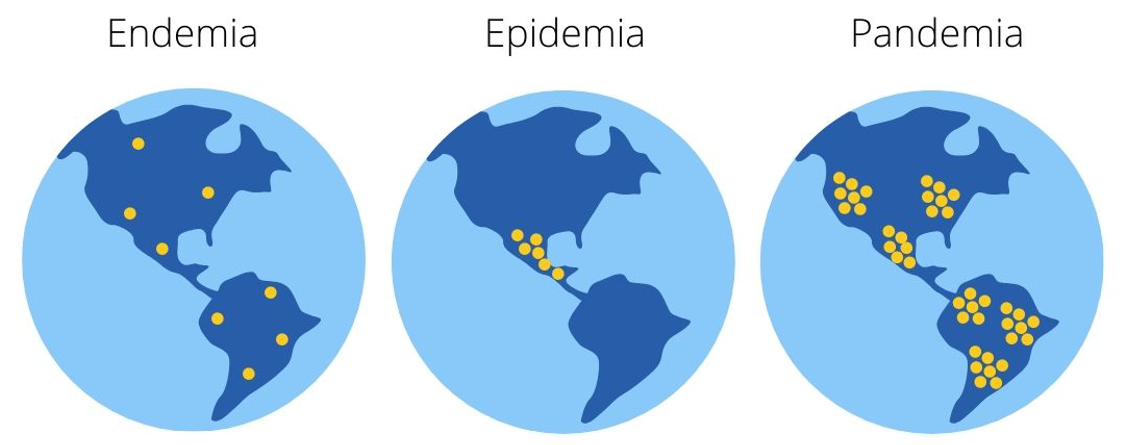
\includegraphics[width=0.7\textwidth]{img/endemia.png}
        \caption{Diferencias entre epidemia, endemia y pandemia.}
        \label{fig:difernecias}
        \vspace{0.5cm} % Ajusta el espacio vertical entre la imagen y el texto
    \end{figure}


\section{Modelos epidemiológicos  deterministas}

\subsection{Modelos epidemiologícos}
Los modelos epidemiológicos son herramientas matemáticas y computacionales que permiten representar de manera simplificada los procesos biológicos, sociales y ambientales que influyen en la propagación de enfermedades dentro de una población. Estos modelos describen cómo las enfermedades infecciosas (y, en algunos casos, no infecciosas) se transmiten entre individuos y cómo varía el estado de salud de la población a lo largo del tiempo \cite{ferrero2021modelos}.

En términos generales, un modelo epidemiológico intenta captar las dinámicas clave del contagio, recuperación, inmunidad, nacimiento y muerte, mediante el uso de ecuaciones diferenciales, teoría de probabilidades o simulaciones computacionales. Dependiendo de su complejidad, pueden incorporar factores como heterogeneidad en la población, movilidad, redes de contacto, y respuesta a intervenciones sanitarias.

Entre los objetivos principales de los modelos epidemiológicos se encuentran:
\begin{itemize}
    \item Describir la dinámica de transmisión de enfermedades en poblaciones susceptibles, entender cómo y por qué una enfermedad se propaga o desaparece.
    \item Estimar parámetros clave como la duración de la infección, la tasa de transmisión, número básico de reproducción R0 y la proporción de población que debe ser vacunada para llegar a alcanzar la inmunidad colectiva.
    \item Explorar escenarios hipotéticos, permitiendo simular diversas condiciones y prever la evolución en el tiempo de una epidemia bajo diferentes supuestos.
    \item Evaluar estrategias de intervención y control como vacunación, cuarentena, aislamiento de casos, uso de mascarillas, cierre de escuelas. permiten calcular el impacto potencial de estas medidas antes de aplicarlas.
    \item Guiar decisiones en salud pública, ofreciendo soporte cuantitativo para la toma de decisiones en contextos de brotes, pandemias o planificación preventiva.
    \item Comprender el impacto de factores sociales y demográficos, como la densidad poblacional, la movilidad geográfica, la estructura etaria o el comportamiento humano, sobre la propagación de enfermedades.
    \item Contribuir al diseño de políticas sanitarias efectivas, mediante la identificación de puntos críticos donde las intervenciones pueden ser más eficaces o eficientes.
\end{itemize}

Los modelos epidemiológicos pueden clasificarse, entre otros criterios, según la ausencia o presencia de aleatoriedad:
\begin{itemize}
    \item \textbf{Deterministas}, aquellos en los que la evolución del fenómeno depende de manera unívoca del conjunto de condiciones iniciales y de los parámetros establecidos. Es decir, no existe aleatoriedad en el proceso, si se repite el modelo con los mismos valores, el resultado será siempre el mismo. Este tipo de modelos se basa habitualmente en ecuaciones diferenciales y resulta útil para analizar el comportamiento general de una enfermedad en poblaciones grandes, donde se busca una aproximación global y reproducible de un fenómeno.
    \item \textbf{Estocásticos}, incorporan procesos aleatorios, lo que implica que, aun con el mismo conjunto de variables y parámetros, la solución del modelo puede variar en cada ejecución. Esto permite captar mejor la variabilidad inherente a fenómenos reales, especialmente en contextos donde las poblaciones son pequeñas o existe un alto grado de incertidumbre.
\end{itemize}
	
Para el desarrollo del este trabajo se ha elegido el uso de modelos deterministas, dado que permiten describir de manera clara y estructurada la evolución de una enfermedad en función de condiciones iniciales y parámetros conocidos. Este enfoque facilita el análisis matemático y la interpretación de los resultados. Además, es útil cuando se trabaja con poblaciones grandes y se busca comprender el comportamiento general de propagación de una enfermedad.

\subsection{Modelos epidemiológicos detrministas}
Por lo tanto, los modelos epidemiológicos deterministas son herramientas matemáticas que permiten describir la propagación de una enfermedad en una población mediante un conjunto de ecuaciones diferenciales. Su principal característica es que, dadas unas condiciones iniciales y unos parámetros fijos, el comportamiento del modelo es completamente predecible y reproducible. Es decir, no hay presencia de azar, los resultados siempre serán los mismos si se parte de las mismas condiciones. Este enfoque resulta especialmente útil para analizar epidemias a gran escala, ya que proporciona una visión general del comportamiento dinámico de la enfermedad y permite evaluar el impacto potencial de distintas intervenciones sanitarias, como la vacunación o el aislamiento.

Dentro del enfoque determinista, existen distintos modelos clásicos que se utilizan para representar diversas realidades epidemiológicas en función de las características del agente infeccioso y de la inmunidad que genera. Estos modelos se conocen como modelos compartimentales, ya que dividen a la población en distintos compartimentos o grupos, cada uno de los cuales representa un estado específico frente a la enfermedad, como susceptibles, infectados, recuperados, etc. La dinámica de la enfermedad se modela a través del flujo de individuos entre estos compartimentos, de acuerdo con tasas de transición establecidas por las ecuaciones del modelo.

Los principales modelos que se estudiarán en este trabajo son: SI, SIS, SIR y SEIR. En este apartado se ofrecerá una descripción general de cada uno, mientras que un análisis más detallado y riguroso se presentará posteriormente en el apartado dedicado a la metodología. Todo de lo que se ha hablado se puede encontrar en el libro \cite{allen2008mathematical}.

\subsubsection*{Modelo SI}
El primero modelo determinista clásico que se puede considerar, representa la forma más simple de modelar una enfermedad infecciosa. A pesar de su sencillez, resulta útil para comprender los principios básicos de la dinámica de contagio en casos dende no existe recuperación ni inmunidad.

El modelo SI (Susceptibles-Infectados) divide a la población en dos grupos: los individuos susceptibles (S), que pueden contraer la enfermedad, y los infectados (I), que ya han contraído la enfermedad y pueden transmitirla. Este modelo asume que una vez que una personas se infecta permanece en este estado indefinidamente, sin posibilidad de recuperación.


\subsubsection*{Modelo SIS}
El modelo SIS (Susceptibles – Infectados) es un modelo que se emplea para representar enfermedades infecciosas que no generar inmunidad tras la recuperación. Una vez que el individuo infectado se recupera, no desarrolla protección duradera frente a la enfermedad, por lo que vuelve a ser susceptible y puede volver a infectarse.

Este comportamiento es característico de algunas enfermedades producidas por bacterias o por protozoos. En estos casos, la respuesta inmunitaria del organismo no es suficiente para prevenir futuras infecciones, especialmente en contextos donde la exposición al agente patógeno es continua o recurrente.
El modelo SIS mantiene la estructura básica del modelo SI, con dos compartimentos:
\begin{itemize}
    \item S (Susceptibles): individuos que pueden contraer la enfermedad.
    \item I (Infectados): individuos que están enfermos y pueden transmitir la infección.
\end{itemize}

La principal diferencia con respecto al modelo SI es que el modelo SIS introduce un flujo de regreso desde el compartimento I al S, representando la recuperación sin inmunidad. Esto implica que los infectados, tras un cierto periodo de tiempo, pasan nuevamente al grupo de susceptibles, reiniciando el ciclo de contagio.
Este modelo es especialmente útil para estudiar enfermedades endémicas, en las que la infección se mantiene de forma constante en una población, y donde la reinfección es frecuente. También permite analizar el equilibrio dinámico entre los individuos infectados y susceptibles en el largo plazo.


\subsubsection*{Modelo SIR}
El modelo SIR (Susceptibles – Infectados – Recuperados) es un modelo clásico ampliamente utilizado en epidemiología para representar la propagación de enfermedades infecciosas que generan inmunidad tras la recuperación. A diferencia del modelo SIS, en el que los individuos recuperados vuelven a ser susceptibles, el modelo SIR asume que una vez que un individuo se recupera, desarrolla inmunidad duradera y que no puede volver a infectarse.

Este comportamiento es característico de muchas infecciones virales como el sarampión, la varicela o la gripe estacional, así como de otras enfermedades para las cuales existen mecanismos inmunológicos eficaces, ya sea naturales o adquiridos mediante vacunación.

El modelo SIR divide la población en tres compartimentos:
\begin{itemize}
    \item S (Susceptibles): individuos que pueden contraer la enfermedad.
    \item I (Infectados): individuos que están infectados y pueden transmitir el patógeno.
    \item R (Recuperados): individuos que han superado la infección y han adquirido inmunidad.
\end{itemize}

La dinámica del modelo SIR se basa en el paso progresivo de los individuos desde el estado susceptible al infectado y, posteriormente, al recuperado. La tasa de transmisión ($\beta$) determina la velocidad a la que los susceptibles se infectan, mientras que la tasa de recuperación ($\gamma$) determina cuánto tarda un individuo en pasar del estado infectado al recuperado.

Este modelo es especialmente útil para analizar epidemias agudas, donde tras un brote inicial se alcanza un pico de infecciones, seguido de un descenso conforme aumenta el número de personas inmunizadas. Además, el modelo permite calcular el número básico de reproducción, indica el promedio de personas que un infectado puede contagiar en una población totalmente susceptible.


\subsubsection*{Modelo SEIR}
El modelo SEIR (Susceptibles – Expuestos – Infectados – Recuperados) es una extensión del modelo clásico SIR que añade un compartimento adicional para capturar de forma más realista el comportamiento de muchas enfermedades infecciosas: el estado expuesto (E). Este modelo es especialmente útil para enfermedades que tienen un periodo de incubación, durante el cual los individuos ya están infectados, pero aún no presentan síntomas ni son contagiosos. 

En el modelo SEIR, la población se divide en cuatro compartimentos:
\begin{itemize}
    \item S (Susceptibles): individuos sanos que pueden contraer la enfermedad.
    \item E (Expuestos): individuos que han sido infectados, pero aún no son contagiosos (fase de incubación).
    \item I (Infectados): individuos que ya pueden transmitir la enfermedad.
    \item R (Recuperados): individuos que se han curado y han adquirido inmunidad.
\end{itemize}
	
Este modelo permite reflejar con mayor precisión el retraso entre la exposición al virus y el momento en que una persona se vuelve infecciosa, algo que no se contempla en el modelo SIR. La dinámica del modelo se basa en las siguientes tasas:
\begin{itemize}
    \item ~$\beta$ (tasa de transmisión): probabilidad de que una persona susceptible se exponga al virus al entrar en contacto con un infectado.
    \item ~$\sigma$ (tasa de progresión o incubación): ritmo al que los individuos expuestos pasan a estar infectados.
    \item $\gamma$ (tasa de recuperación): velocidad con la que los infectados se recuperan y adquieren inmunidad.
\end{itemize}

El modelo SEIR es especialmente relevante cuando se necesita considerar el impacto del periodo de incubación en la propagación de la enfermedad. Esta capacidad lo convierte en una herramienta esencial para el análisis y predicción de brotes epidémicos más complejos, así como para evaluar el efecto de medidas de control tempranas, como el aislamiento preventivo o cuarentena.

A pesar de ser una simplificación de la realidad, el modelo SEIR ofrece una aproximación más ajustada que el modelo SIR para muchas infecciones reales, permitiendo a epidemiólogos y responsables sanitarios diseñar estrategias más eficaces de intervención y prevención.





\section{Vacunación}
\subsection{Importancia}
La vacunación, figura, constituye una de las intervenciones más eficaces y trascendentales en la historia de la salud pública. Ha permitido prevenir la propagación de enfermedades infecciosas, reducir de forma significativa la morbilidad y la mortalidad asociadas, y, a veces, erradicar por completo determinadas patologías. Según estimaciones de la OMS\footnote{Organización Muncial de la Salud} \cite{oms_vacunas}, la vacunación previene entre 3 y 5 millones de muertes anuales causadas por enfermedades. Gracias a los programas de inmunización masiva, millones de vidas se salvan cada año, y muchas enfermedades han sido controladas de forma notable. En el contexto de las epidemias, no solo protege a los individuos vacunados, sino que también contribuye a la inmunidad colectiva o de grupo, lo cual reduce la transmisión comunitaria y protege a las personas que no pueden vacunarse, como los inmunocomprometidos o niños demasiado pequeños. Además de los beneficios en salud, la vacunación genera impactos económicos y sociales significativos según \cite{nandi2020vaccines}: reduce los costes médicos, disminuye la carga sobre los sistemas sanitarios y mejora la productividad al minimizar las pérdidas. La vacunación universal, tanto rutinaria como de recuperación, es un componente crítico de la atención médica de calidad.


\subsection{Tipos}
Existen diferentes formas de clasificar la vacunación como se explica en \cite{hhs_vaccines} y se puede ver en la tabla \ref{tab:tipos_vacunacion}.

\begin{table}[H]
\centering
\caption{Clasificación de los tipos de vacunación}
\label{tab:tipos_vacunacion}
\begin{tabularx}{\textwidth}{|l|X|}
\hline
\textbf{Criterio} & \textbf{Tipos de vacunación} \\
\hline
Según la finalidad &
Vacunación preventiva \\
& Vacunación terapéutica \\
\hline
Según la estrategia poblacional &
Vacunación rutinaria \\
& Vacunación de campaña \\
& Vacunación selectiva \\
& Vacunación masiva \\
\hline
Según el tipo de vacuna &
Vacunas inactivadas \\
& Vacunas atenuadas \\
& Vacunas conjugadas \\
& Vacunas recombinantes \\
& Vacunas de ARNm \\
& Vacunas vectoriales \\
\hline
\end{tabularx}
\end{table}


\subsection{Evolución e historia}
La historia de la vacunación es un recorrido fundamental en el desarrollo de la medicina y la salud pública. Se remonta a observaciones empíricas sobre la inmunidad natural tras ciertas enfermedades. En 1796, \textbf{Edward Jenner} desarrolló la primera vacuna al utilizar material de pústulas de vacas infectadas con viruela bovina para prevenir la viruela humana, marcando el inicio de la vacunación moderna \cite{damaso2018revisiting}.

Durante el siglo XIX, \textbf{Louis Pasteur} realizó importantes aportes al crear vacunas utilizando formas atenuadas de microorganismos, desarrollando inmunizaciones contra enfermedades como la rabia. Su trabajo, junto con la teoría microbiana de la enfermedad y las investigaciones de \textbf{Robert Koch}, permitió el desarrollo de vacunas contra la tuberculosis, la difteria y otras enfermedades infecciosas \cite{schwartz2022pasteurian}.

En el siglo XX, los avances en biotecnología, como el cultivo celular, posibilitaron la producción de vacunas contra enfermedades como la poliomielitis, el sarampión, las paperas y la rubéola. Posteriormente, la biología molecular permitió el desarrollo de vacunas recombinantes, como la vacuna contra la hepatitis B.

En la actualidad, la tecnología de ARN mensajero ha revolucionado la vacunación, facilitando el desarrollo rápido de vacunas.





\subsection{Impacto y desafíos actuales}
A pesar del impacto positivo y ampliamente documentado de la vacunación, según \cite{lindstrand2021world}persisten diversos desafíos que afectan su implementación y sostenibilidad a nivel global:
\begin{itemize}
    \item \textbf{Hesitación vacunal y desconfianza}: la desinformación, las creencias en métodos alternativos o "naturales" y la falta de confianza en los sistemas sanitarios generan una baja aceptación de las vacunas en ciertos grupos. 
    \item \textbf{Desigualdades en el acceso}: en regiones de bajos ingresos, existen barreras económicas, logísticas y estructurales que dificultan la distribución equitativa de vacunas. Iniciativas como \textbf{\textit{GAVI}}\footnote{Global Alliance for Vaccines and Immunisation, consorcio internacional compuesto por diversas entidades objetivo es facilitar el acceso a vacunas en países menos desarrollados}, han mejorado la situación, pero aún persisten importantes brechas.
    \item \textbf{Infraestructura limitada}: los sistemas de salud en países de ingresos bajos suelen carecer del personal capacitado, recursos financieros y logística necesarios para mantener programas de vacunación sostenibles.
    \item \textbf{Impacto de la pandemia de COVID-19}: la crisis sanitaria interrumpió programas de vacunación rutinaria, reduciendo las tasas de cobertura y aumentando la exposición a enfermedades prevenibles.
    \item \textbf{Resurgimiento de enfermedades}: La disminución en la cobertura vacunal ha provocado brotes recientes de enfermedades. La OMS insiste en la necesidad de mantener altas tasas de cobertura para prevenir estas situaciones.
\end{itemize}



\section{SIDA/VIH}
Según \cite{sudharshan2008introduction} el síndrome de inmunodeficiencia adquirida (SIDA)  es una enfermedad causada por la infección del virus de la inmunodeficiencia humana (VIH). El VIH es un retrovirus que ataca y destruye las células CD4+T, esenciales para el sistema inmunológico, lo que provoca una inmunodeficiencia progresiva. Las personas infectadas se vuelven más susceptibles a infecciones y ciertos tipos de cáncer. La estructura del VIH se observa en la figura \ref{fig:vih estructura}\footnote{Obtenida de \cite{infosida_vih}}

\begin{figure}[H]
    \centering
    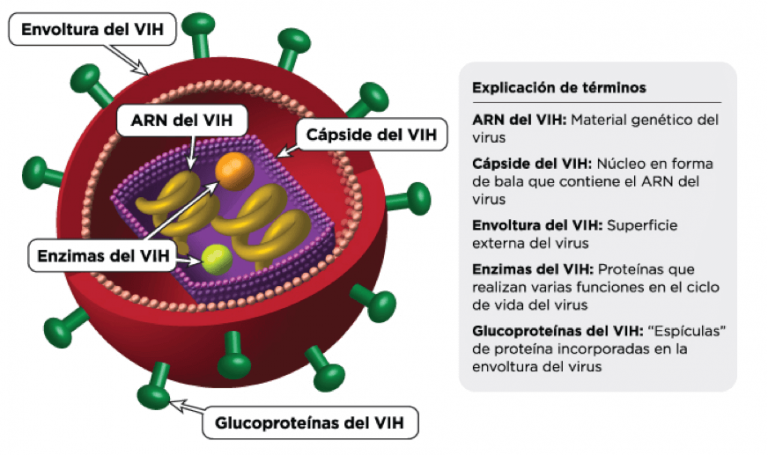
\includegraphics[width=0.7\textwidth]{img/vih_estructura.png}
    \caption{Estrucutura del virus de la inmunodeficiencia humana (VIH)}
    \label{fig:vih estructura}
    \vspace{0.5cm} % Ajusta el espacio vertical entre la imagen y el texto
\end{figure}

\subsection{Vías de transmisión}
El VIH se transmite a través de varias vías bien definidas, como se explica en \cite{shaw2012hiv}:
\begin{itemize}
    \item Contacto sexual: principal forma de transmisión. Ocurre en relaciones sexuales sin protección, mediante fluidos infectados.
    \item Uso compartido de agujas: entre personas usuarias de drogas intravenosas. Alto riesgo por la introducción directa del virus en la sangre.
    \item Transfusiones de sangre y productos sanguíneos: aunque posible, su riesgo es mínimo en países donde se realizan pruebas rigurosas en bancos de sangre.
    \item Transmisión madre-hijo: puede ocurrir durante el embarazo, parto o lactancia. El uso de TAR\footnote{Terapia Antirretroviral} y cesáreas programadas reduce el riesgo.
    \item Trasplantes de órganos: es raro debido a los controles.
    \item Exposición ocupacional: riesgo bajo en profesionales de la salud si se siguen las precauciones adecuadas.
\end{itemize}

\subsection{Diagnóstico}
El diagnóstico se basa en:
\begin{enumerate}
    \item Inmunoensayo combinado Ag/Ab: detecta anticuerpos contra VIH y antígeno p24. Puede identificar la infección 2–3 semanas después de la exposición \cite{workowski2021sexually}.
    \item Prueba de diferenciación de anticuerpos.
    \item Prueba de amplificación de ácidos nucleicos (NAAT): se emplea si hay resultados indeterminados. \cite{saag2021hiv}.
    \item Pruebas rápidas: Ofrecen resultados preliminares en menos de 20 minutos. Se deben confirmar con pruebas de laboratorio.
\end{enumerate}

\subsection{Tratamiento}
El tratamiento se basa en TAR \cite{heendeniya2019antiretroviral}, que ha convertido al VIH en una enfermedad crónica controlable.

\textbf{Opciones terapéuticas}. Según \cite{sivanandy2023efficacy} los INSTI\footnote{Inhibidores de la transferencia de cadena de la integrasa} constituyen la primera línea de tratamiento. Además, se utilizan terapias de acción prolongada.

\textbf{Consideraciones clínicas}. Según \cite{saag2021hiv} entre los efectos secundarios se incluyen náuseas, cefaleas, acidosis láctica y hepatomegalia con esteatosis. Es fundamental ajustar el tratamiento considerando la función renal y hepática del paciente, así como posibles interacciones medicamentosas.

\textbf{Impacto psicosocial}. El estigma asociado puede afectar negativamente la adherencia al tratamiento y la calidad de vida de los pacientes. El apoyo psicológico y social resulta esencial para mejorar su bienestar  \cite{cihlar2016current}.

\subsection{Estrategias de prevención}
Su prevención \cite{chan2012biomedical} combina medidas farmacológicas, no farmacológicas y de salud pública.

\textbf{Enfoques farmacológicos}.
La PrEP\footnote{Profilaxis preexposición} consiste en el uso diario de antirretrovirales en personas con alto riesgo de contraer el virus. La PEP\footnote{Profilaxis postexposición} implica la administración inmediata de antirretrovirales tras una posible exposición. Además, el TasP\footnote{Tratamiento como prevención} se basa en que las personas con carga viral indetectable no transmiten el virus (indetectable = intransmisible).

\textbf{Enfoques no farmacológicos}.
Se encuentra el uso de preservativos, circuncisión masculina, educación para promover prácticas sexuales seguras, y programas de intercambio de agujas que disminuyen la transmisión entre usuarios de drogas intravenosas.

\textbf{Medidas de salud pública}.
Incluyen el diagnóstico temprano para iniciar el tratamiento oportuno, la prevención de la transmisión de madre a hijo mediante intervenciones médicas, e intervenciones para reducir desigualdades sociales.

\subsection{Progresión clínica}
Tras la infección inicial, se observan tres fases:
\begin{enumerate}
    \item \textbf{Fase aguda}: síntomas similares a los de una gripe.
    \item \textbf{Fase de latencia clínica}: puede durar años; el paciente es asintomático mientras el virus se replica en niveles bajos.
    \item \textbf{Progresión a SIDA}: ocurre como se explica en \cite{okoye2013cd} cuando el recuento de CD4+ cae por debajo de 200 células/µL o aparecen infecciones oportunistas como sarcoma de Kaposi o candidiasis esofágica.
\end{enumerate}
La media del tiempo entre la infección y el desarrollo de SIDA en ausencia de tratamiento es de 8 a 10 años. Factores como la carga viral, coinfecciones o la respuesta inmune individual influyen en la progresión \cite{hoover1992progression}.

\subsection{Evolución e impacto}
Desde los años 80, el impacto del SIDA ha cambiado significativamente gracias al desarrollo de TARGA\footnote{Terapia antirretroviral de gran actividad}. La incidencia de enfermedades oportunistas se redujo drásticamente, pasando de 30.7 a 2.5 casos por cada 100 años-paciente entre 1994 y 1998, según el estudio EuroSIDA\footnote{estudio observacional de cohortes prospectivo que sigue a personas con VIH} \cite{mocroft2000aids}. Además, se ha observado un aumento en el recuento de células CD4+ en los diagnósticos recientes, lo que indica un mejor manejo clínico de la enfermedad. Sin embargo, el impacto del SIDA no ha sido uniforme, ha habido un aumento de infecciones en mujeres, jóvenes y minorías. Los avances en pruebas diagnósticas, como las pruebas rápidas orales, han facilitado la detección temprana del VIH, aunque persisten desafíos importantes, como el diagnóstico tardío \cite{san2003incidence}.
En la figura \ref{fig:evolución vih}\footnote{Obtenido en \cite{madrid_salud_poblacion}} se puede observar la evolución en la Comunidad de Madrid 

\begin{figure}[H]
    \centering
    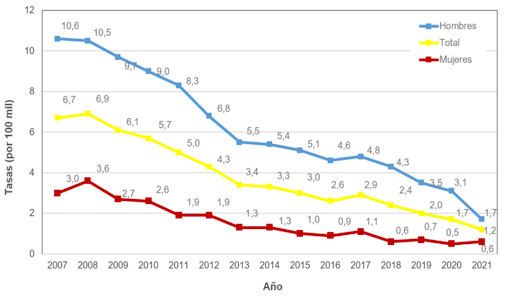
\includegraphics[width=0.7\textwidth]{img/evolucionVIH.png}
    \caption{Evolución VIH en la Comunidad de Madrid de 2007 a 2021}
    \label{fig:evolución vih}
    \vspace{0.5cm} % Ajusta el espacio vertical entre la imagen y el texto
\end{figure}

\section{Gonorrea}
La gonorrea según \cite{unemo2019gonorrhoea} es una infección o enfermedad de transmisión sexual causada por la bacteria \textit{Neisseria gonorrhoeae}. De las más comunes a nivel mundial, con una incidencia anual estimada de 86.9 millones de casos en adultos.


\subsection{Vías de transmisión}
Se transmite principalmente a través del contacto sexual sin protección \cite{workowski2021sexually}. Durante las relaciones sexuales vaginales, puede infectar el tracto genital tanto en hombres como en mujeres. En las relaciones anales, la infección puede afectar el recto. Asimismo, durante el sexo oral sin protección, puede colonizar la faringe.

Otra vía, la perinatal, en la cual una madre infectada puede transmitir la bacteria a su bebé durante el parto. Posibilidad de transmisión al utilizar saliva como lubricante, especialmente entre hombres que tienen sexo con hombres. 

\subsection{Diagnóstico}
Debe considerar las posibles infecciones en el tracto urogenital, recto y faringe. Los métodos principales incluyen  NAAT\footnote{Pruebas de amplificación de ácidos nucleicos}, cultivo bacteriano y tinción de Gram incluidos en \cite{adamson2022diagnostic}.

Las NAAT son el estándar de oro (gold standard) debido a su alta sensibilidad y especificidad. Permiten el uso de diferentes tipos de muestras. Ventaja de facilitar el autodiagnóstico mediante muestras autocolectadas por los pacientes.

El cultivo bacteriano, aunque menos sensible, es fundamental para la detección de cepas resistentes a los antimicrobianos. Requiere muestras como las uretrales, endocervicales, rectales, faríngeas o conjuntivales, y es útil para realizar pruebas de susceptibilidad en casos de fracaso del tratamiento.

La tinción de Gram puede ser diagnóstica en hombres sintomáticos cuando se observan diplococos gramnegativos intracelulares en secreciones uretrales. Sin embargo, su sensibilidad es menor en mujeres y en sitios extragenitales, por lo que no se recomienda como única prueba diagnóstica en estos casos.

La combinación de estos métodos permite un diagnóstico oportuno y efectivo, lo que es clave para el tratamiento adecuado y la prevención de complicaciones y nuevas transmisiones.

\subsection{Tratamiento}
La gonorrea ha desarrollado resistencia a múltiples antibióticos. Actualmente, el tratamiento recomendado según \cite{cyr2020update} es una dosis única de ceftriaxona, con la posible adición de doxiciclina si no se ha descartado coinfección por Chlamydia trachomatis.

Debido al aumento de la resistencia a medicamentos \cite{unemo2019antimicrobial}, es fundamental la vigilancia continua de la eficacia de los tratamientos. En caso de sospecha de fallo terapéutico, se recomienda realizar pruebas de susceptibilidad, especialmente en infecciones faríngeas. La investigación actual se centra en el desarrollo de nuevos antimicrobianos y vacunas para combatir la resistencia emergente.

\subsection{Prevención}
Estrategias recomendadas incluidas en \cite{mayor2012diagnosis} son:
\begin{itemize}
    \item Uso correcto de preservativos.
    \item Educación y consejería sobre prácticas sexuales seguras y reducción de riesgos.
    \item Detección y tratamiento de parejas sexuales para evitar reinfecciones y transmisión. 
    \item Cribado regular.
    \item Promoción de salud pública, acceso a servicios, reducción del estigma y políticas efectivas.
\end{itemize}

\subsection{Clínica y complicaciones}
Los síntomas varían según el sexo \cite{unemo2019gonorrhoea}. En los hombres, se manifiesta como uretritis con disuria y secreción purulenta. En las mujeres, muchas veces asintomática, aunque puede presentarse como cervicitis con secreción mucopurulenta y dolor pélvico.

Las complicaciones también difieren. En las mujeres, puede derivar en enfermedad inflamatoria pélvica, infertilidad, embarazo ectópico y dolor crónico. En los hombres, la principal complicación es la epididimitis, que también puede conllevar infertilidad. En ambos sexos, existe el riesgo de desarrollar una infección gonocócica diseminada. Las infecciones extragenitales incluyen proctitis, faringitis que suele ser asintomática y conjuntivitis neonatal cuando ocurre transmisión perinatal.

Desde el punto de vista de la salud pública, la gonorrea incrementa el riesgo de transmisión del VIH. Además, la creciente resistencia a los antimicrobianos representa un desafío significativo para su control y tratamiento.

\subsection{Historia y evolución}
La gonorrea ha sido una infección de transmisión sexual prevalente durante miles de años. Desde la introducción de los antibióticos, ha desarrollado resistencia progresiva. Primero se observó con las sulfonamidas y penicilinas en las décadas de 1940 y 1950. Posteriormente, surgió resistencia a las tetraciclinas y macrólidos, y más tarde a las fluoroquinolonas durante las décadas de 1980 y 1990. En la actualidad, la terapia recomendada que anteriormente incluía el uso dual de ceftriaxona y azitromicina también enfrenta un aumento preocupante en la resistencia, con casos reportados de cepas resistentes a ambos antibióticos. \cite{golparian2020genomic}.

Esta evolución subraya la necesidad de desarrollar nuevas estrategias y medidas de prevención para controlar la propagación de esta infección \cite{lin2021epidemiology}.
En la figura \ref{fig:evolución gonorrea} obtenida de \cite{isanidad2023}, se observa como ha evolucionado la gonorrea en España, donde se ve que los casos han aumentado, una causa puede ser la resitencia a los antibióticos.

\begin{figure}[H]
    \centering
    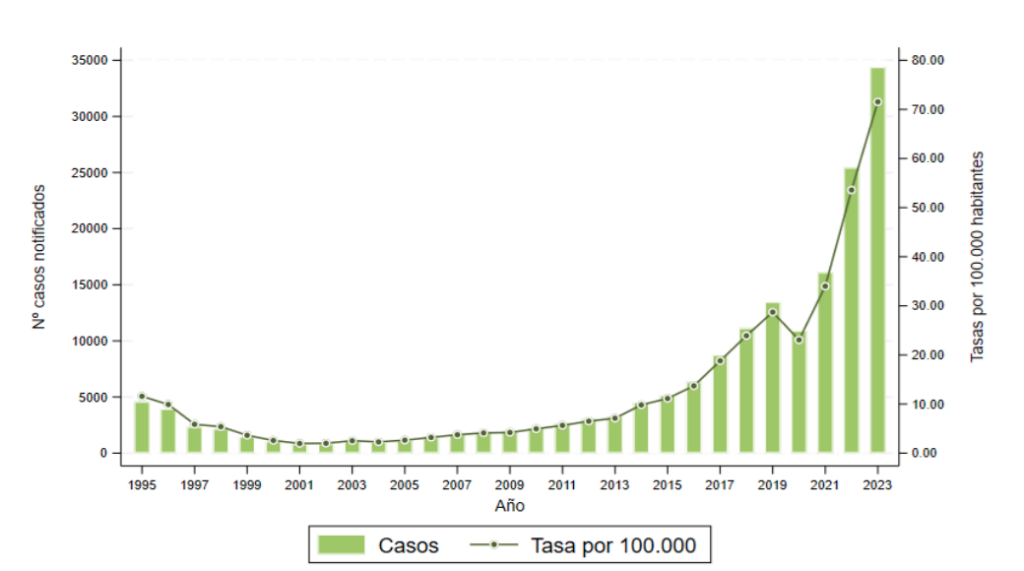
\includegraphics[width=0.7\textwidth]{img/incidenciagonorrea.png}
    \caption{Evolución gonorrea en España de 1995 a 2023}
    \label{fig:evolución gonorrea}
    \vspace{0.5cm} % Ajusta el espacio vertical entre la imagen y el texto
\end{figure}


\section{Sarampión}
El sarampión según \cite{workowski2021sexually}es una enfermedad vírica altamente contagiosa, causada por el MeV\footnote{Virus del sarampión}. Antes de la introducción de la vacuna, prácticamente todos los niños la contraían durante la infancia. La transmisión se produce por vía respiratoria. Se caracteriza por fiebre, tos, coriza, conjuntivitis y exantema maculopapular, se observa en la figura \ref{fig:sarampión}\footnote{Obtenida de \cite{tododiagnostico2020sarampion}}.

\begin{figure}[H]
        \centering
        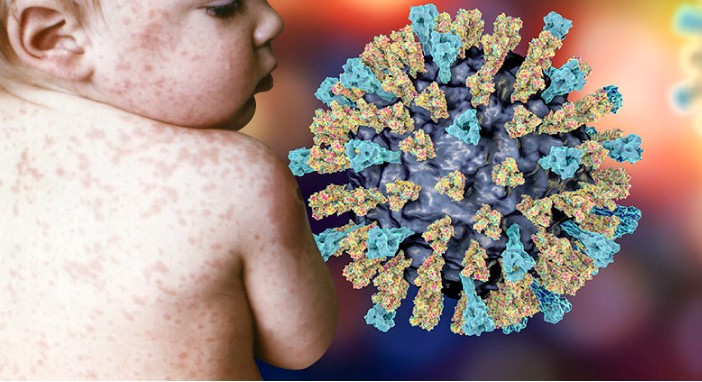
\includegraphics[width=0.7\textwidth]{img/sarampion.jpg}
        \caption{Representación del virus del sarampión (MeV) junto a la manifestación clínica típica de la enfermedad exantema maculopapular}
        \label{fig:sarampión}
        \vspace{0.5cm} % Ajusta el espacio vertical entre la imagen y el texto
\end{figure}

\subsection{Vías de transmisión}
Se transmite a través de gotitas respiratorias y por vía aérea mediante núcleos de gotas aerosolizadas. Las personas infectadas son contagiosas desde cuatro días antes hasta cuatro días después de la aparición del exantema. Es una de las enfermedades víricas más contagiosas conocidas. Los seres humanos son el único huésped natural del virus del sarampión, lo que hace factible su erradicación a nivel global \cite{moss2017measles}.

\subsection{Diagnóstico}
El diagnóstico se basa \cite{baeten2012antiretroviral} en una combinación de criterios clínicos y confirmación mediante pruebas de laboratorio.

\textbf{Presentación clínica}: el sarampión se caracteriza por fiebre, exantema maculopapular y al menos uno de los tres signos clásicos: tos, coriza y conjuntivitis. Un hallazgo clínico Las manchas de Koplik, pequeñas lesiones blanquecinas en la mucosa bucal que aparecen antes del exantema.

\textbf{Confirmación de laboratorio}:
\begin{enumerate}
    \item Detección de anticuerpos IgM específicos contra el virus del sarampión: método más común y se realiza mediante ELISA\footnote{Ensayo de inmunoadsorción ligado a enzima}. Los anticuerpos IgM pueden no ser detectables en las primeras 72 horas tras la aparición del exantema, aunque casi siempre están presentes después de 4 días.
    \item RT-PCR\footnote{PCR de transcripción inversa}: identificar material genético del virus en diferentes muestras. Útil en las etapas tempranas, antes de que se desarrollen los anticuerpos IgM. Permite la genotipificación del virus, que facilita el seguimiento epidemiológico de su propagación.
    \item Seroconversión de IgG:  se utiliza con menor frecuencia debido a la disponibilidad limitada de pruebas cuantitativas de IgG en muchos laboratorios clínicos locales.
\end{enumerate}

\subsection{Tratamiento}
Las intervenciones terapéuticas clave en el artúclo \cite{graber2020update} son las siguientes.

\textbf{Terapia de soporte}.
Hidratación y control de los síntomas, a través del uso de antipiréticos y otros cuidados generales.

\textbf{Suplementación con vitamina A}.
La OMS recomienda su administración en todos los casos agudos en niños, con el objetivo de reducir el riesgo de complicaciones.
Dosis orales administradas una vez al día durante dos días. En casos de deficiencia clínica de vitamina A, se recomienda una tercera dosis.

\textbf{Tratamiento de infecciones bacterianas secundarias}.
Puede predisponer a infecciones bacterianas como la neumonía. Administrar antibióticos adecuados, según la infección y la susceptibilidad del paciente.

\textbf{Aislamiento y prevención de la transmisión}.
Los pacientes deben ser aislados para evitar la transmisión del virus. Implementar medidas de control, como uso de mascarillas.

\subsection{Prevención}
Puede prevenirse mediante la vacunación. Se administra en formulaciones combinadas, como la SRP (sarampión, paperas y rubéola) se muestra en la figura \ref{fig:vacuna sarampión}\footnote{Obtenida de \cite{aarp_sarampion_2019}} o la SRPV (que también incluye varicela), ha demostrado ser segura y efectiva.

\begin{figure}[H]
        \centering
        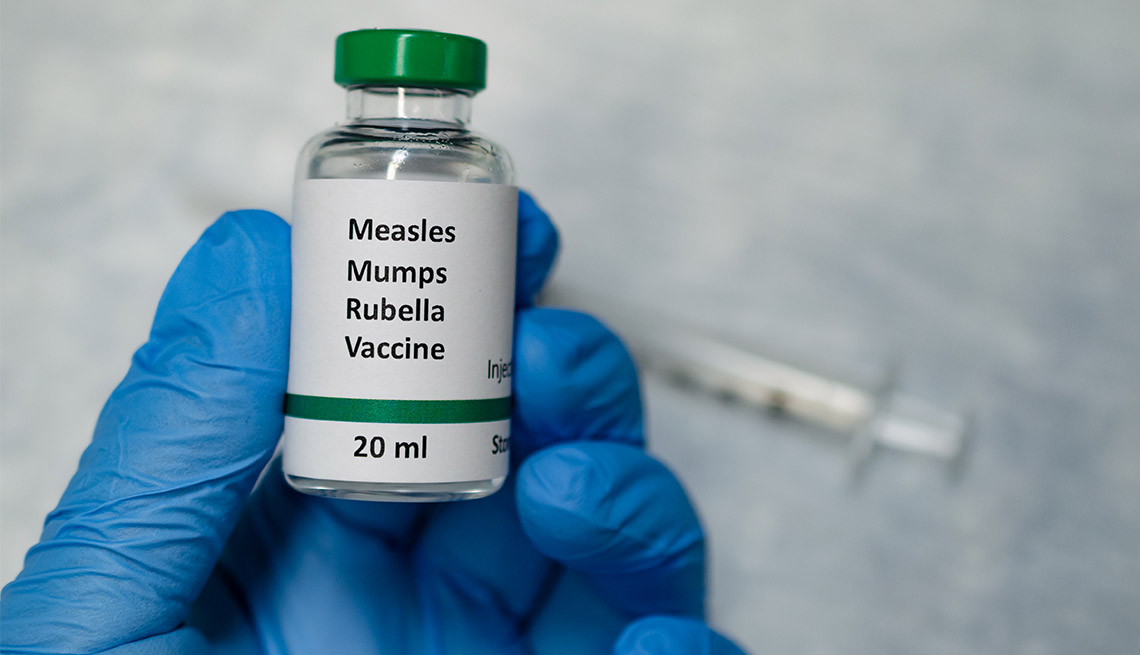
\includegraphics[width=0.7\textwidth]{img/vacunaMMR.jpg}
        \caption{Vacuna triple de sarampión, paperas y rubeola, siglas inglés MMV}
        \label{fig:vacuna sarampión}
        \vspace{0.5cm} % Ajusta el espacio vertical entre la imagen y el texto
\end{figure}

Se recomienda la administración de dos dosis de la vacuna SRP: la primera entre los 12 y 15 meses de edad y la segunda entre los 4 y 6 años \cite{gastanaduy2021measles}. Debe priorizarse la vacunación en grupos con mayor riesgo de exposición, como estudiantes, personal sanitario o viajeros internacionales.
En personas susceptibles, la administración de la vacuna dentro de las 72 horas tras la exposición puede prevenir. Alternativamente, la inmunoglobulina humana puede administrarse hasta 6 días después, especialmente en lactantes, embarazadas no inmunizadas y personas inmunodeprimidas. Dado que la inmunoglobulina proporciona una inmunidad temporal, se recomienda completar la vacunación con SRP.

\subsection{Progeresión clínica y complicaciones}
Evolución clínica característica, dividida en varias fases como se explica en \cite{cdc_measles}:
\begin{enumerate}
    \item \textbf{Fase prodrómica}: dura de 2 a 4 días, incluye fiebre, tos, coriza y conjuntivitis. Manchas de Koplik.
    \item \textbf{Fase exantemática}: alrededor de 14 días tras la exposición, exantema maculopapular que comienza en la cara y se extiende, persistiendo entre 4 y 7 días.
    \item \textbf{Recuperación}: en casos no complicados, el exantema desaparece en orden inverso a su aparición y la recuperación completa se da en torno a una semana después.
\end{enumerate}

Puede ocasionar complicaciones graves, especialmente en niños pequeños, adultos mayores, embarazadas, personas desnutridas o inmunocomprometidas. Las más frecuentes son: otitis media, neumonía, diarrea, encefalitis o SSPE \footnote{Panencefalitis esclerosante subaguda}.

\subsection{Impacto histórico y situación actual}
Ha tenido un impacto significativo en la salud pública mundial. Antes de la introducción de la vacuna, era una enfermedad endémica que afectaba a la mayoría de los niños y causaba millones de muertes al año. Con la llegada de la vacunación, su incidencia disminuyó. Entre 2000 y 2017, los casos a nivel global se redujeron en un 83\%, y las muertes anuales pasaron de 545 mil a 109 mil como se destaca en \cite{shanks2014measles}. 
Sigue siendo una causa importante de mortalidad infantil en regiones con baja cobertura vacunal y sistemas de salud frágiles. La reaparición de brotes se ha asociado a la desinformación y la disminución de las tasas de vacunación \cite{fischer2016zinc}.

En la figura \ref{fig:evolución sarampión}\footnote{Obtenida de \cite{ahumada2015modelos}}, se muestra un ejemplo del caso de Chile, evolución del sarampión entre los años 1939 y 2014. Notable disminución de la enfermedad a partir de la introducción de la vacuna, con una caída aún más significativa tras la implementación de campañas de vacunación, hasta alcanzar su eliminación.

\begin{figure}[H]
        \centering
        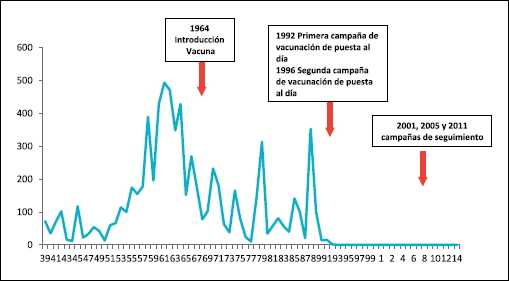
\includegraphics[width=0.7\textwidth]{img/evolucionSarampion.jpg}
        \caption{Tasa de incidencia de sarampión en Chile 1939-2014, asociado a inclusión de la vacuna y campañas de vacunación.}
        \label{fig:evolución sarampión}
        \vspace{0.5cm} % Ajusta el espacio vertical entre la imagen y el texto
\end{figure}

\section{COVID-19}
El COVID-19\footnote{Enfermedad por coronavirus} es causada por el virus SARS-CoV-2 figura \ref{fig:covid estructura}\footnote{Obtenida de \cite{medlineplus_sarscov2}}, altamente transmisible que surgió a finales de 2019 en Wuhan, China. Su transmisión se produce a través de gotículas respiratorias generadas al hablar, toser o estornudar, durante el contacto cercano. No obstante, también puede propagarse mediante aerosoles en espacios cerrados, así como por contacto con superficies contaminadas.

\begin{figure}[H]
        \centering
        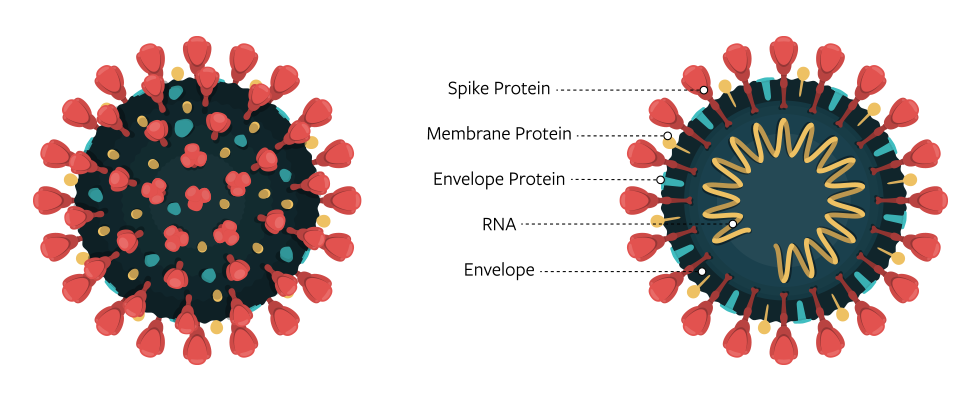
\includegraphics[width=0.7\textwidth]{img/estructuracovid.png}
        \caption{Estructura del virus SARS-CoV-2 (COVID-19).}
        \label{fig:covid estructura}
        \vspace{0.5cm} % Ajusta el espacio vertical entre la imagen y el texto
\end{figure}

\subsection{Vías de transmsión}
Según \cite{wiersinga2020covid19}existen varios mecanismos de transmisión:
\begin{itemize}
    \item Gotas respiratorias: partículas de mayor tamaño que se depositan rápidamente, facilitando la transmisión a corta distancia.
    \item Aerosoles: partículas más pequeñas que pueden permanecer suspendidas en el aire, en espacios cerrados y mal ventilados, permitiendo la transmisión a mayor distancia.
    \item Fómites: aunque el virus puede sobrevivir en superficies inanimadas durante horas o días, forma de contagio menos frecuente.
    \item Transmisión asintomática: individuos sin síntomas pueden transmitir el virus, especialmente en las fases presintomáticas, contribuye a su propagación.
\end{itemize}

\subsection{Diagnóstico}
Se fundamenta principalmente \cite{ko2022covid} en la detección del ARN del SARS-CoV-2 mediante pruebas moleculares, especialmente la RT-PCR, considerada el método de referencia por su alta sensibilidad y especificidad.

\textbf{RT-PCR}: se realiza sobre muestras respiratorias y permite detectar el virus en fases tempranas.

\textbf{Pruebas de antígenos}: aunque menos sensibles, ofrecen resultados rápidos y son útiles en entornos donde se requiere diagnóstico inmediato.

\textbf{Pruebas serológicas}: detectan anticuerpos y son útiles para estudios epidemiológicos, pero no para el diagnóstico en fases agudas.

\subsection{Tratamiento}
Varía según la gravedad del cuadro clínico. En casos leves o moderados, se basa en medidas como el reposo, la hidratación, el control de la fiebre y el dolor, y el seguimiento domiciliario. En pacientes con factores de riesgo, se recomienda un monitoreo más estrecho para detectar complicaciones \cite{qaseem2023outpatient}. En casos graves, requieren hospitalización y soporte respiratorio, incluyendo oxigenoterapia. Se emplean tratamientos específicos para reducir la inflamación, prevenir complicaciones como la trombosis, y mejorar la respuesta inmunitaria. En algunos casos, es necesario el ingreso en UCI y el uso de ventilación mecánica \cite{wiersinga2020pathophysiology}.

\subsection{Medidas de prevención}
Las principales medidas para prevenir el COVID-19 incluidas en \cite{hutchins2020covid}:
\begin{itemize}
    \item Vacunación, herramienta más eficaz para reducir la gravedad de la enfermedad. Se recomienda para todas las personas mayores de 6 meses.
    \item Uso de mascarilla, útil en espacios cerrados, especialmente en situaciones de alta transmisión.
    \item Distanciamiento físico y ventilación, mantener una distancia adecuada y mejorar la ventilación en interiores.
    \item Higiene de manos: lavarse frecuentemente con agua y jabón o usar gel hidroalcohólico.
    \item Recomendaciones para personas de alto riesgo, además de las medidas generales, deben mantenerse al día con las dosis de refuerzo, considerar el uso de antivirales tras una exposición y monitorizar su estado de salud en casa. En caso de infección, deben seguir las recomendaciones de aislamiento.
\end{itemize} 
Estas estrategias, combinadas, son clave para reducir la transmisión y proteger a la población más vulnerable.

\subsection{Progresión clínica}
La evolución varía desde formas asintomáticas hasta cuadros críticos. Generalmente se explica en \cite{cdc_covid19_yellowbook} que sigue estas fases:

\begin{enumerate}
    \item Incubación e inicio: el periodo de 2 a 14 días. Los síntomas iniciales incluyen fiebre, tos, malestar, dolor de garganta. La pérdida del olfato y gusto es frecuente.
    \item Fase prodrómica (1ª semana): síntomas respiratorios leves o moderados. Neumonía incipiente y alteraciones leves en marcadores inflamatorios.
    \item Fase aguda (2ª semana): se intensifican los síntomas. Complicaciones como neumonía grave, daño cardíaco o trastornos de coagulación. Los marcadores inflamatorios y hematológicos alcanzan sus niveles más alterados.
    \item Fase de remisión (3ª semana): los síntomas comienzan a mejorar, aunque la inflamación puede persistir.
    \item Convalecencia, la recuperación puede tardar semanas, dependiendo de la gravedad del cuadro.
\end{enumerate}

Factores de riesgo: edad avanzada, enfermedades crónicas y alteraciones inmunológicas aumentan el riesgo de enfermedad grave. Hallazgos clínicos, en casos graves, se observan linfopenia y elevación de marcadores como dímero D, PCR y ferritina. Las imágenes pulmonares suelen mostrar opacidades en vidrio esmerilado.

\subsection{Impacto de la pandemia del COVID-19}
Ha tenido consecuencias profundas a nivel global, afectando múltiples aspectos de la sociedad. 
\begin{itemize}
\item Salud pública. Con más de 774 millones de casos y 7 millones de muertes hasta febrero de 2024, la incidencia se puede observar en la figura \ref{fig:muertes covid}\footnote{Obtenida de \cite{elpais_covidmap}}, la pandemia desbordó los sistemas de salud, generando escasez de recursos y personal médico, especialmente en poblaciones vulnerables.
\begin{figure}[H]
        \centering
        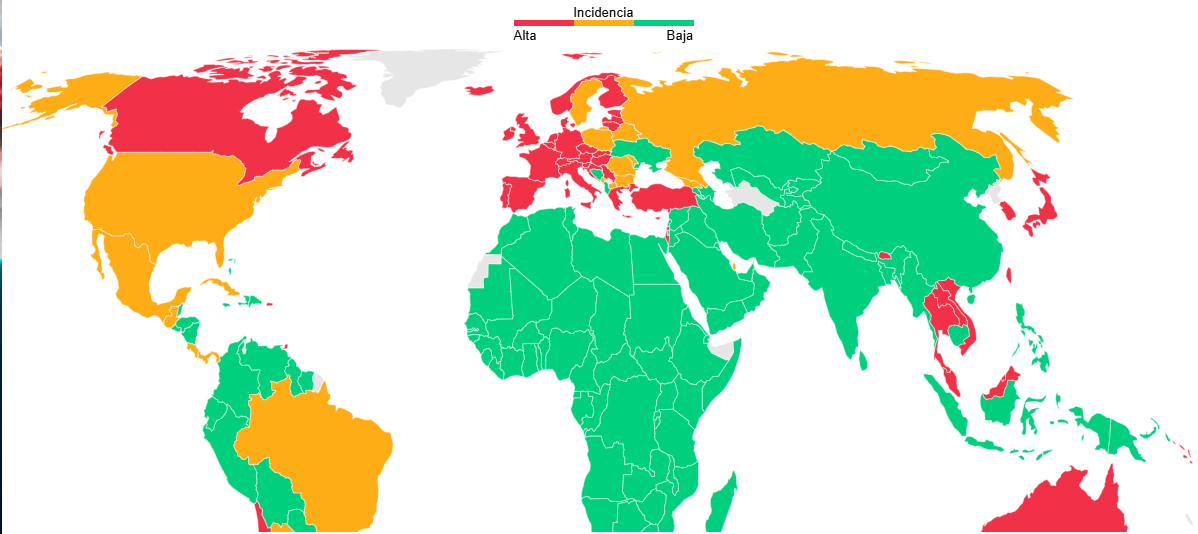
\includegraphics[width=0.7\textwidth]{img/covid_muertes.png}
        \caption{Distribución global de la incidencia de muertes hasta el 2 de febrero de 2025, categorizada por intensidad: baja (verde), media (naranja) y alta (rojo).}
        \label{fig:muertes covid}
        \vspace{0.5cm} % Ajusta el espacio vertical entre la imagen y el texto
\end{figure}

    \item Economía. El confinamiento y cierre de actividades afectaron gravemente sectores como el turismo, la hostelería y el comercio, y acentuando las desigualdades económicas.
    \item Vida social y salud mental. El aislamiento y la incertidumbre aumentaron niveles de ansiedad, depresión y otros trastornos mentales, al tiempo que se intensificaron el estigma y la discriminación hacia ciertos grupos.
    \item Educación. El cierre de centros educativos forzó una transición abrupta a la educación en línea, revelando y ampliando las brechas digitales.
    \item Medio ambiente. La reducción de la actividad humana durante los confinamientos produjo efectos positivos temporales, como la disminución de emisiones contaminantes y la mejora en la calidad del aire.
\end{itemize}

La pandemia evidenció vulnerabilidades globales y la necesidad de fortalecer sistemas sanitarios, reducir desigualdades y prepararse mejor para futuras emergencias \cite{miyah2022covid}.

\section{Ingeniería de control}
La ingeniería de control es una disciplina de la ingeniería que se encarga del análisis y diseño de sistemas capaces de autorregularse para alcanzar comportamientos deseados. Su objetivo es influir sobre el comportamiento dinámico de un sistema, ante ciertas entradas o perturbaciones, se obtenga una respuesta predefinida, deseable o estable \cite{tme_ingenieria_control}. Se apoya en la teoría de control, que proporciona las herramientas para analizar cómo los sistemas responden a estímulos y cómo diseñar mecanismos para modificar esa respuesta. Los sistemas controlados pueden ser físicos, químicos, biológicos o sociales, y todos ellos comparten una estructura común, poseen entradas, salidas, variables de estado y, en muchos casos, un mecanismo de retroalimentación.

El concepto de \textbf{retroalimentación} es central en esta disciplina. Un sistema con retroalimentación mide continuamente su salida y la compara con un valor deseado (referencia). Realiza ajustes automáticos en sus entradas para minimizar el error. Otro de los principios clave es la \textbf{estabilidad del sistema}. Un sistema es estable si, ante una perturbación o cambio en las condiciones iniciales, tiende a volver a su estado de equilibrio o comportamiento deseado sin intervención externa constante. Mientras que un sistema inestable puede presentar comportamientos no deseados, como respuestas crecientes o caóticas, que requieren intervención activa o rediseño del sistema de control \cite{ait_ingenieria_control}.


\textbf{La regulación mediante PID\footnote{Proporcional-Integral-Derivativo}} es una técnica ampliamente utilizada en el control automático de sistemas para mantener una variable de proceso, como la temperatura, velocidad o presión, en un valor deseado o setpoint. Un controlador PID ajusta la señal de control basándose en tres acciones \cite{mazzone2002controladores}:
\begin{itemize}
    \item Proporcional (P): corrige el error actual multiplicándolo por una ganancia proporcional.
    \item Integral (I): considera la acumulación del error pasado para eliminar el error constante a largo plazo.
    \item Derivativa (D): anticipa la tendencia futura del error, basándose en su tasa de cambio, para mejorar la estabilidad y respuesta del sistema.
\end{itemize}

Combinando estas tres acciones, el controlador PID puede responder rápidamente a cambios, reducir errores y minimizar oscilaciones, logrando un control eficiente y preciso en múltiples aplicaciones industriales y tecnológicas.


\subsection{Relación con los modelos epidemiologicos deterministas}
La ingeniería de control, aunque más utilizada en campos como la ingeniería mecánica o eléctrica, ha encontrado aplicaciones cada vez más relevantes en áreas como la biomedicina, la salud pública y la epidemiología. En este sentido, el estudio y la gestión de enfermedades infecciosas pueden abordarse desde una perspectiva de sistemas dinámicos, donde se aplican conceptos de la teoría de control para modelar, analizar y diseñar estrategias de intervención. En el contexto de enfermedades como el sarampión o el COVID-19, la población afectada y las tasas de contagio, recuperación o vacunación pueden representarse mediante modelos matemáticos dinámicos como SIR o SEIR. Estos modelos funcionan como sistemas que evolucionan en el tiempo, respondiendo a entradas externas como campañas de vacunación, cambios de comportamiento social o aparición de nuevas variantes del virus.

Desde la ingeniería de control, las estrategias de \textbf{vacunación masiva} pueden interpretarse como acciones de control diseñadas para modificar el comportamiento del sistema (epidemia) y llevarlo hacia un estado deseado (como una incidencia cercana a cero). En este caso, el sistema de salud actúa como el controlador que mide la evolución de la epidemia (salida) y ajusta las intervenciones (entrada) en función de los resultados observados.
Además, el concepto de \textbf{retroalimentación} se refleja en la toma de decisiones basadas en datos epidemiológicos. Por ejemplo, si se observa un aumento en el número de contagios, el sistema sanitario puede responder con un aumento de las medidas preventivas como más vacunación o confinamientos. Este lazo de control permite estabilizar la situación sanitaria y evitar comportamientos incontrolables en la propagación de la enfermedad.
También se puede hablar de \textbf{estabilidad epidemiológica}: un sistema sanitario bien diseñado busca que, incluso ante perturbaciones como la llegada de nuevos brotes, la incidencia no se dispare, sino que el sistema sea capaz de amortiguar el impacto y regresar a una situación de control. Aquí es donde la ingeniería de control y la salud pública convergen en una visión interdisciplinaria y estratégica.

Incluir el enfoque de la ingeniería de control en el estudio de enfermedades infecciosas no solo permite describir su comportamiento dinámico, sino también diseñar y evaluar políticas de intervención eficaces y sostenibles. La modelización y control de epidemias ofrece terreno para la aplicación de herramientas de ingeniería con impacto directo en la salud pública.

\section{Estado del arte y trabajos relacionados}
En esta sección se presenta una revisión actualizada sobre el uso de modelos deterministas en el estudio de la propagación de enfermedades infecciosas, con especial atención a los modelos SIS, SIR y SEIR, así como sus variantes que incorporan estrategias de vacunación. La revisión se estructura de forma cronológica y temática, destacando los enfoques teóricos, las aportaciones aplicadas y los trabajos que han influido directamente en el desarrollo del presente proyecto. Para cada estudio se identifican los elementos técnicos más relevantes y su aplicabilidad a esta investigación, que incluye además la implementación de los modelos mediante la herramienta Simulink.

\textbf{Los modelos compartimentales deterministas}, como SI, SIR, SIS y SEIR, han sido fundamentales en la comprensión de la propagación de enfermedades infecciosas. Introducidos por Kermack y McKendrick en 1927 \cite{brauer2005kermack}, estos modelos dividen la población en compartimentos según el estado de la enfermedad y describen las transiciones entre ellos mediante EDO\footnote{Ecuaciones diferenciales ordinarias}. Por ejemplo, el modelo SIR considera tres compartimentos: Susceptibles (S), Infectados (I) y Recuperados (R), y ha sido ampliamente utilizado para enfermedades como el sarampión y la gripe \cite{carcione2020simulation}.

Estudios recientes han extendido estos modelos para incluir dinámicas más complejas. Se han incorporado nacimientos y muertes, inmunidad temporal, vacunación y heterogeneidad poblacional. Un ejemplo de ello es el modelo SEIRS, que añade un compartimento de Expuestos (E) y considera la pérdida de inmunidad, permitiendo que los individuos recuperados vuelvan a ser susceptibles \cite{trawicki2017deterministic}. Estos modelos han sido aplicados para estudiar enfermedades como el VIH y el Ébola, proporcionando información valiosa sobre la dinámica de transmisión y el impacto de las intervenciones.

Sin embargo, es importante reconocer las limitaciones de estos modelos. La suposición de una población homogénea y la omisión de factores estocásticos pueden llevar a sobreestimaciones del número básico de reproducción $R_0$ y a una representación simplificada de la realidad \cite{ali2024deterministic}. Por ello, se han desarrollado modelos estocásticos y enfoques basados en redes para capturar la variabilidad y complejidad de las epidemias reales \cite{islam2020integer}.


\textbf{Simulink}, se ha utilizado para implementar modelos epidemiológicos debido a su capacidad para representar sistemas dinámicos mediante EDO. Su interfaz gráfica facilita la construcción y comprensión de modelos compartimentales, permitiendo a los usuarios simular la evolución temporal de epidemias bajo diferentes escenarios y parámetros.

Existen diversos recursos y ejemplos de implementación de modelos SIR y SEIR en Simulink. Por ejemplo, el proyecto SimCOVID disponible en MATLAB Central proporciona una plataforma para simular la propagación de COVID-19 utilizando modelos compartimentales, permitiendo ajustar parámetros como la tasa de transmisión y la de recuperación para analizar diferentes escenarios \cite{abdulrahman_simcovid_2020}. Asimismo, otros estudios han utilizado Simulink para explorar el impacto de intervenciones como la vacunación y el distanciamiento social en la dinámica de las epidemias \cite{valentini2020sir}.

La implementación en Simulink ofrece ventajas como la facilidad para realizar análisis de sensibilidad, probar diferentes estrategias de control y visualizar los resultados de manera intuitiva. Sin embargo, también presenta desafíos, como la necesidad de una comprensión sólida de las EDO y la correcta parametrización del modelo para reflejar adecuadamente la realidad epidemiológica \cite{wang2020global}.























\capitulo{4}{Metodología}
Los modelos y simulaciones que desarrollados a continuación tienen como finalidad representar de forma simplificada el comportamiento de ciertas enfermedades infecciosas mediante sistemas dinámicos deterministas. A partir de datos reales, se emplean distintos modelos epidemiológicos clásicos para estudiar su evolución en diferentes contextos.

Además, se incorporan modificaciones a algunos de estos modelos con el objetivo de evaluar el impacto de estrategias de control, siendo la vacunación la medida principal. La metodología empleada no solo busca describir la propagación de la enfermedad, sino también explorar posibles formas de mitigarla.


Se ha optado por la simplificación de los modelos para su implementación en Simulink ya que 
en la formulación original de los modelos epidemiológicos, se trabaja con proporciones respecto a la población total, lo que implica definir las fracciones susceptibles e infectadas como se oberva en \eqref{prop}:

\begin{equation}
    S_f = \frac{S}{N}, \quad I_f = \frac{I}{N}
\label{prop}
\end{equation}

Donde \( N \) representa la población total. La tasa de variación de la fracción susceptible se expresa como \eqref{ene}:

\begin{equation}
    \frac{dS_f}{dt} = -\beta_f \cdot I_f \cdot S_f
\label{ene}
\end{equation}

Sustituyendo las fracciones por sus expresiones en términos absolutos \eqref{absolitos}.

\begin{equation}
    \frac{d}{dt} \left( \frac{S}{N} \right) = -\beta_f \cdot \frac{I}{N} \cdot \frac{S}{N}
\label{absolitos}
\end{equation}

Lo que implica \eqref{impli}:

\begin{equation}
    \frac{1}{N} \cdot \frac{dS}{dt} = -\beta_f \cdot \frac{I \cdot S}{N^2}
\label{impli}
\end{equation}

Multiplicando ambos lados por \( N \) \eqref{multi}:

\begin{equation}
    \frac{dS}{dt} = -\left( \frac{\beta_f}{N} \right) \cdot I \cdot S
\label{multi}
\end{equation}

En este punto, se redefine el parámetro beta $\beta$ de transmisión como se oberva en la ecuación \eqref{rede} 

\begin{equation}
    \beta = \frac{\beta_f}{N}
\label{rede}
\end{equation}

Lo cual permite reescribir la ecuación \eqref{final} de forma más compacta, sin necesidad de hacer referencia explícita a la población total.

\begin{equation}
    \frac{dS}{dt} = -\beta \cdot I \cdot S
\label{final}
\end{equation}

Esta transformación es algébricamente equivalente a la formulación original. Sin embargo, tiene la ventaja de simplificar la implementación en herramientas como \texttt{Simulink}, ya que se trabaja directamente con cantidades absolutas de población, y el efecto del tamaño de la población total queda incorporado dentro del valor del parámetro \( \beta \). Esto permite mantener la coherencia del modelo y facilita su análisis y simulación computacional.





\section{Modelo SI}
El modelo SI es un modelo determinista simple que divide la población en susceptibles (S) e infectados (I). Asume que no hay recuperación, una vez infectado, el individuo permanece infectado de forma permanente. Útil para enfermedades crónicas o sin inmunidad.

\textbf{Supuestos del modelo}. La población total N es contante y homogénea, por lo que no se tienen en cuenta ni nacimientos ni muertes, ya sean por la enfermedad o por otras causas. Por lo tanto, la población susceptible más la infectada es la población total. No existe recuperación, los individuos infectados permanecen en este estado permanentemente. La transmisión de la enfermedad ocurre por contacto entre individuos susceptibles e infectados.

Se muestra una representación esquemática del modelo SI mediante el diagrama de flujo, como se ve en la figura \ref{fig:diagrama SI}.

\begin{figure}[H]
    \centering
    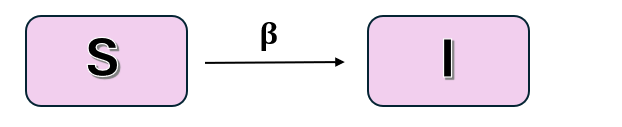
\includegraphics[width=0.7\textwidth]{img/diagrama_SI.png}
    \caption{Diagrama de flujo modelo SI.}
    \label{fig:diagrama SI}
    \vspace{0.5cm} % Ajusta el espacio vertical entre la imagen y el texto
\end{figure}

También se puede describir el modelo a partir del siguiente sistema de ecuaciones diferenciales \eqref{eq:ecuacion 1 Si} \eqref{eq:ecuacion 2 SI}.

\begin{align}
\frac{dS}{dt} &= -\beta SI \label{eq:ecuacion 1 Si} \\
\frac{dI}{dt} &= \beta SI \label{eq:ecuacion 2 SI}
\end{align}

Donde:
\begin{itemize}
    \item 	La ecuación dS⁄dt (\ref{eq:ecuacion 1 Si}), representa la variación del número de personas susceptibles a lo largo del tiempo. Como los individuos susceptibles se van infectando al entrar en contacto con personas contagiadas, este número disminuye progresivamente. Por esta razón, la derivada tiene signo negativo, expresa una pérdida en el grupo de los susceptibles debida al contagio.
    \item 	La ecuación dI⁄dt (\ref{eq:ecuacion 2 SI}), representa la variación del número de personas infectadas en el tiempo. Como los susceptibles que contraen la enfermedad pasan a formar parte del grupo de infectados, este valor aumenta a medida que progresa la transmisión, por lo que la derivada tiene signo positivo.
    \item El parámetro beta ($\beta$) se denomina tasa de transmisión o de contagio. Representa la probabilidad de que un contacto entre un individuo susceptible y uno infectado resulte en un nuevo contagio. Es un valor clave en el modelo, ya que determina la velocidad con la que la enfermedad se propaga por la población. Como se muestra en la ecuación \eqref{eq:beta} tiene unidades inversas al producto de personas y tiempo.
    \begin{equation}
    \beta = \frac{1}{\text{personas} \cdot \text{tiempo}}
    \label{eq:beta}
    \end{equation}
\end{itemize}

 



Este modelo a enfermedad termina por propagarse a toda la población, ya que no tiene cura. Es interesante para enfermedades víricas crónicas, que causan infección de por vida y no tienen cura. La utilidad del modelo es limitada, ya que la mayoría de las enfermedades infecciosas contemplan la recuperación, lo cual no se refleja en este modelo.

El modelo se implementa en Simulink. Para mostrar su funcionamiento y lo que sería un resultado típico de este modelo, se realiza una simulación utilizando datos aleatorios, con el objetivo de observar el comportamiento del modelo SI en un caso práctico, se oberva en la figura \ref{fig:ejemplo SI}. Se considera una población total de 1000 individuos, con 999 personas susceptibles y 1 persona infectada al inicio. La tasa de transmisión es ~$\beta$ = 0,00005. 

\begin{figure}[H]
    \centering
    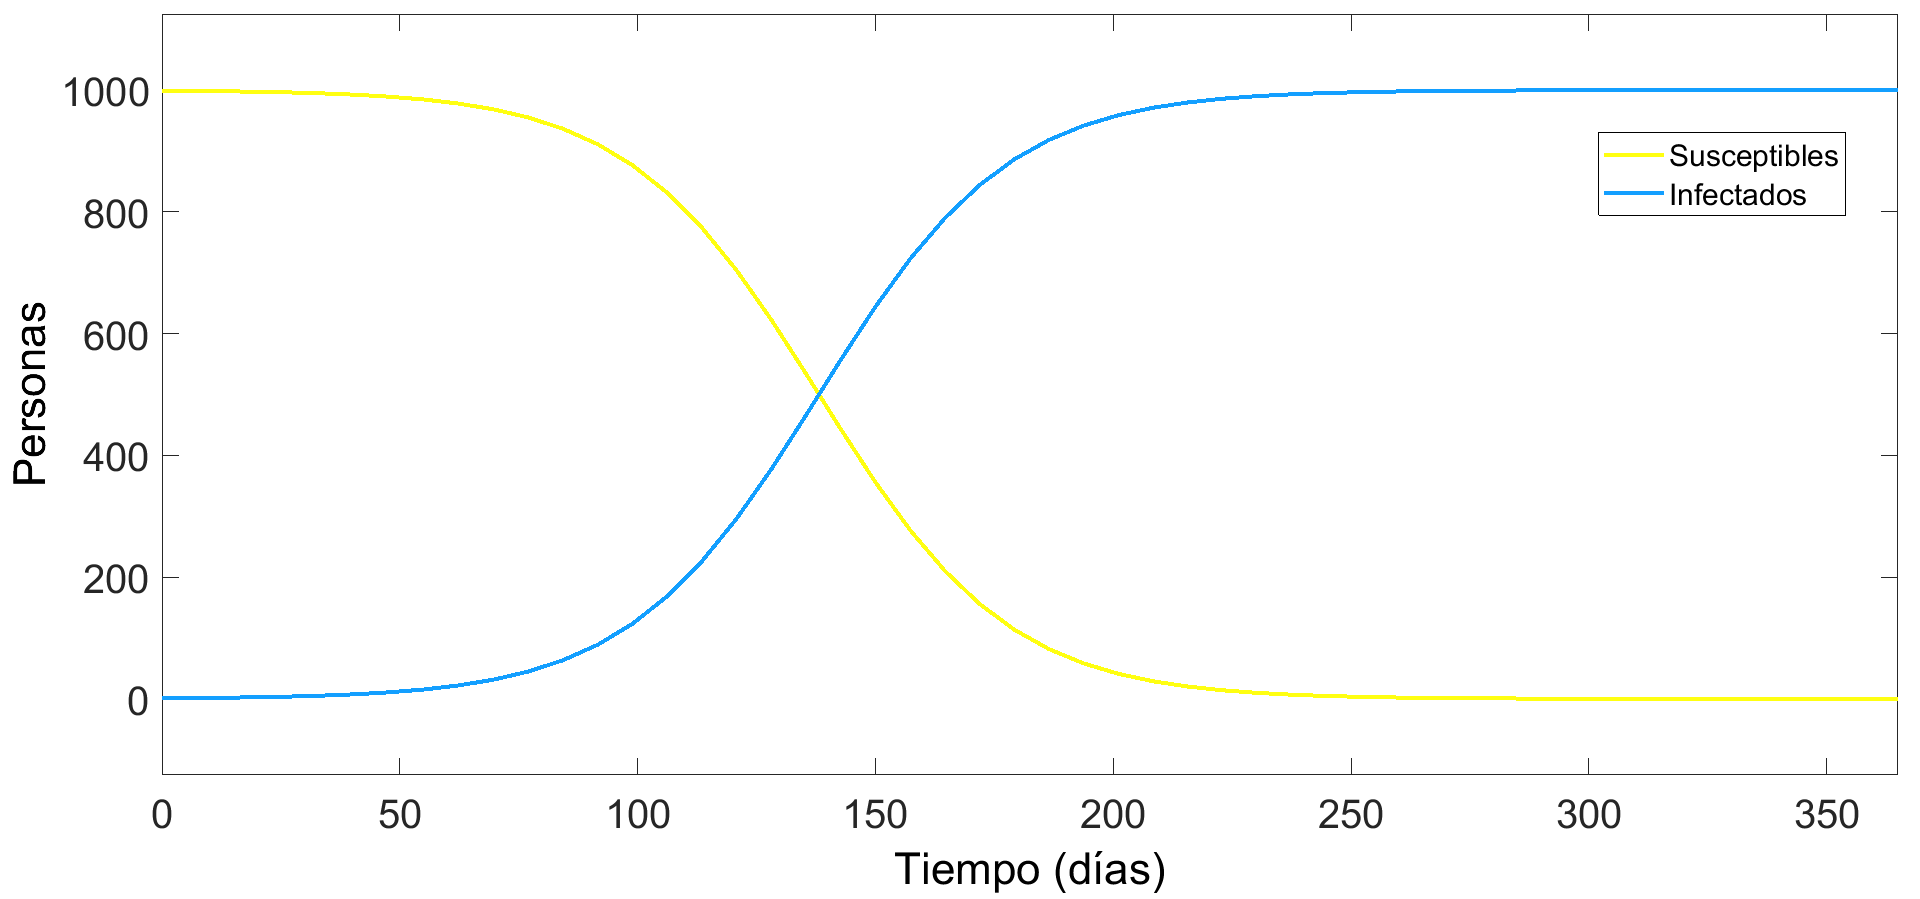
\includegraphics[width=0.7\textwidth]{img/modelo_SI_resultado_ejemplo.png}
    \caption{Resultado típico de un modelo SI.}
    \label{fig:ejemplo SI}
    \vspace{0.5cm} % Ajusta el espacio vertical entre la imagen y el texto
\end{figure}

La figura \ref{fig:ejemplo SI} muestra una disminución en el número de personas susceptibles y un aumento en el número de infectados conforme pasa el tiempo. Inicialmente, casi toda la población es susceptible, lo que permite una propagación acelerada de la enfermedad, especialmente en las primeras etapas, debido a la alta probabilidad de contacto entre infectados y susceptibles.
La dinámica está determinada por la tasa de transmisión $\beta$.
La enfermedad se propaga hasta que toda la población es infectada. Los infectados aumentan hasta que ya no quedan individuos susceptibles.


\section{Número básico de reproducción}
En los modelos compartimentales, analizados a continuación, resulta fundamental el papel del número básico de reproducción, $R_0$, un parámetro clave en epidemiología que permite anticipar el comportamiento de un brote epidémico.

Este parámetro se define como el número medio de infecciones secundarias que un solo individuo infectado es capaz de generar durante todo su periodo de infecciosidad, en una población compuesta exclusivamente por individuos susceptibles. Mide el potencial de propagación de la enfermedad en sus primeras etapas, antes de que otros factores como la inmunidad o la intervención sanitaria influyan en su dinámica.
El número básico de reproducción puede expresarse mediante la relación entre la tasa de transmisión y la de recuperación como se ve en la ecuación \ref{eq:ecR0}.

\begin{equation}
R_0 = \frac{\beta}{\gamma}
\label{eq:ecR0}
\end{equation}

Este coeficiente refleja el equilibrio entre la capacidad de la enfermedad para transmitirse y la velocidad con la que los individuos infectados se recuperan y regresan al estado de susceptibles. 
El valor de $R_0$ es fundamental para predecir la evolución del brote:
\begin{itemize}
    \item Si $R_0$ > 1, cada personas infectada contagia a más de una persona, lo que implica que la enfermedad se propaga y puede llegar a establecerse de forma endémica en la población.
    \item Si $R_0$ < 1, cada infectado genera, de media, menos de un caso nuevo, por lo que la enfermedad tiende a desaparecer con el tiempo.
    \item Si $R_0$ = 1, cada persona infectada reemplaza a otra, manteniendo el número de casos estable, pero sin expansión, no se produce un brote epidémico.
\end{itemize}
	
Cuando una enfermedad alcanza un valor de $R_0$ >1, pero sin provocar un crecimiento exponencial descontrolado, puede establecerse en un estado endémico. Esto significa que la enfermedad permanece presente de forma continua en una población o región determinada, con un número de casos que se mantiene relativamente constante a lo largo del tiempo.

La \textbf{endemicidad} implica que se ha alcanzado un equilibrio entre la transmisión del patógeno y los mecanismos que limitan su propagación, como, la inmunidad parcial de la población, la adaptación del agente patógeno a sus huéspedes y las intervenciones sanitarias o cambios de comportamiento.

Es importante aclarar que el hecho de que una enfermedad sea endémica no significa que sea benigna o que no represente un riesgo para la salud pública. De hecho, muchas enfermedades endémicas siguen teniendo un impacto considerable en términos de morbilidad y mortalidad, y requieren esfuerzos constantes de vigilancia, prevención y control.

\section{Modelo SIS}
El modelo SIS representa enfermedades donde no se adquiere inmunidad tras la recuperación. Los individuos infectados se recuperan y vuelven a ser susceptibles, permitiendo reinfecciones. Es útil para estudiar enfermedades endémicas con contagio recurrente.

\textbf{Supuestos del modelo}. En este modelo también se asume que no ocurren ni nacimientos ni muertes, ya sean por la propia enfermedad o por otras circunstancias.

Se muestra una representación esquemática del modelo SIS mediante el diagrama de flujo, representado en la figura \ref{fig:diagrama SIS}.
\begin{figure}[H]
    \centering
    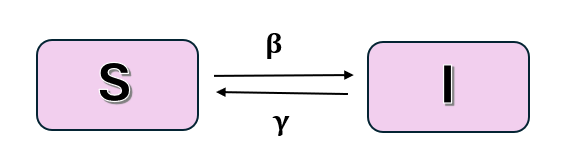
\includegraphics[width=0.7\textwidth]{img/diagrama_SIS.png}
    \caption{Diagrama de flujo modelo SIS.}
    \label{fig:diagrama SIS}
    \vspace{0.5cm} % Ajusta el espacio vertical entre la imagen y el texto
\end{figure}

También se puede representar el modelo mediante el siguiente sistema de ecuaciones diferenciales \eqref{eq:ec1SIS} \eqref{eq:ec2SIS}.

\begin{align}
\frac{dS}{dt} &= -\beta SI + \gamma I \label{eq:ec1SIS} \\
\frac{dI}{dt} &= \beta SI - \gamma I \label{eq:ec2SIS}
\end{align}

Donde:
\begin{itemize}
    \item 	La ecuación dS⁄dt (\ref{eq:ec1SIS}), representa la tasa de cambio de la población susceptible. Esta cantidad disminuye cuando los individuos se infectan, se expresa mediante un término negativo asociado a la tasa de contagio. Sin embargo, también aumenta cuando los individuos infectados se recuperan, ya que no se desarrolla inmunidad y vuelven a ser susceptibles. Por eso la tasa de recuperación aparece con signo positivo.
    \item 	La ecuación dI⁄dt (\ref{eq:ec2SIS}), representa la tasa de cambio de la población infectada. Este valor aumenta como consecuencia de los nuevos contagios, se refleja con término positivo asociado a la tasa de transmisión. A su vez, disminuye cuando los infectados se recuperan y regresan al compartimento de susceptibles, por ello gamma aparece con signo negativo.
    \item 	El parámetro beta ($\beta$), tasa de transmisión o de contagio. Probabilidad de que un contacto entre un individuo susceptible y uno infectado resulte en un nuevo contagio. 
    \item 	El parámetro gamma ($\gamma$) se denomina tasa de recuperación. Indica la probabilidad de que un individuo infectado se recupere y vuelva a ser susceptible, es este contexto. Las unidades de la tasa de recuperación gamma son \[[\text{tiempo}]^{-1}\]  Se interpreta como el inverso del tiempo medio de recuperación \eqref{eq:gammacal}.
    \begin{equation}
    \gamma = \frac{1}{\text{tiempo medio de recuperación}}
    \label{eq:gammacal}
    \end{equation}
\end{itemize}


El modelo se implementa en Simulink. Para mostrar su funcionamiento y lo que sería un resultado típico de este modelo, se realiza una simulación utilizando datos aleatorios, con el objetivo de observar el comportamiento del modelo SIS en un caso práctico, se observa en la figura \ref{fig:ejeSIS}. Se tiene una población total de 1000 personas, de las cuales 990 son susceptibles y 10 son infectados. La tasa de transmisión es $\beta$ = 0,0003. 
Y la tasa de recuperación es de 0,1.



\begin{figure}[H]
    \centering
    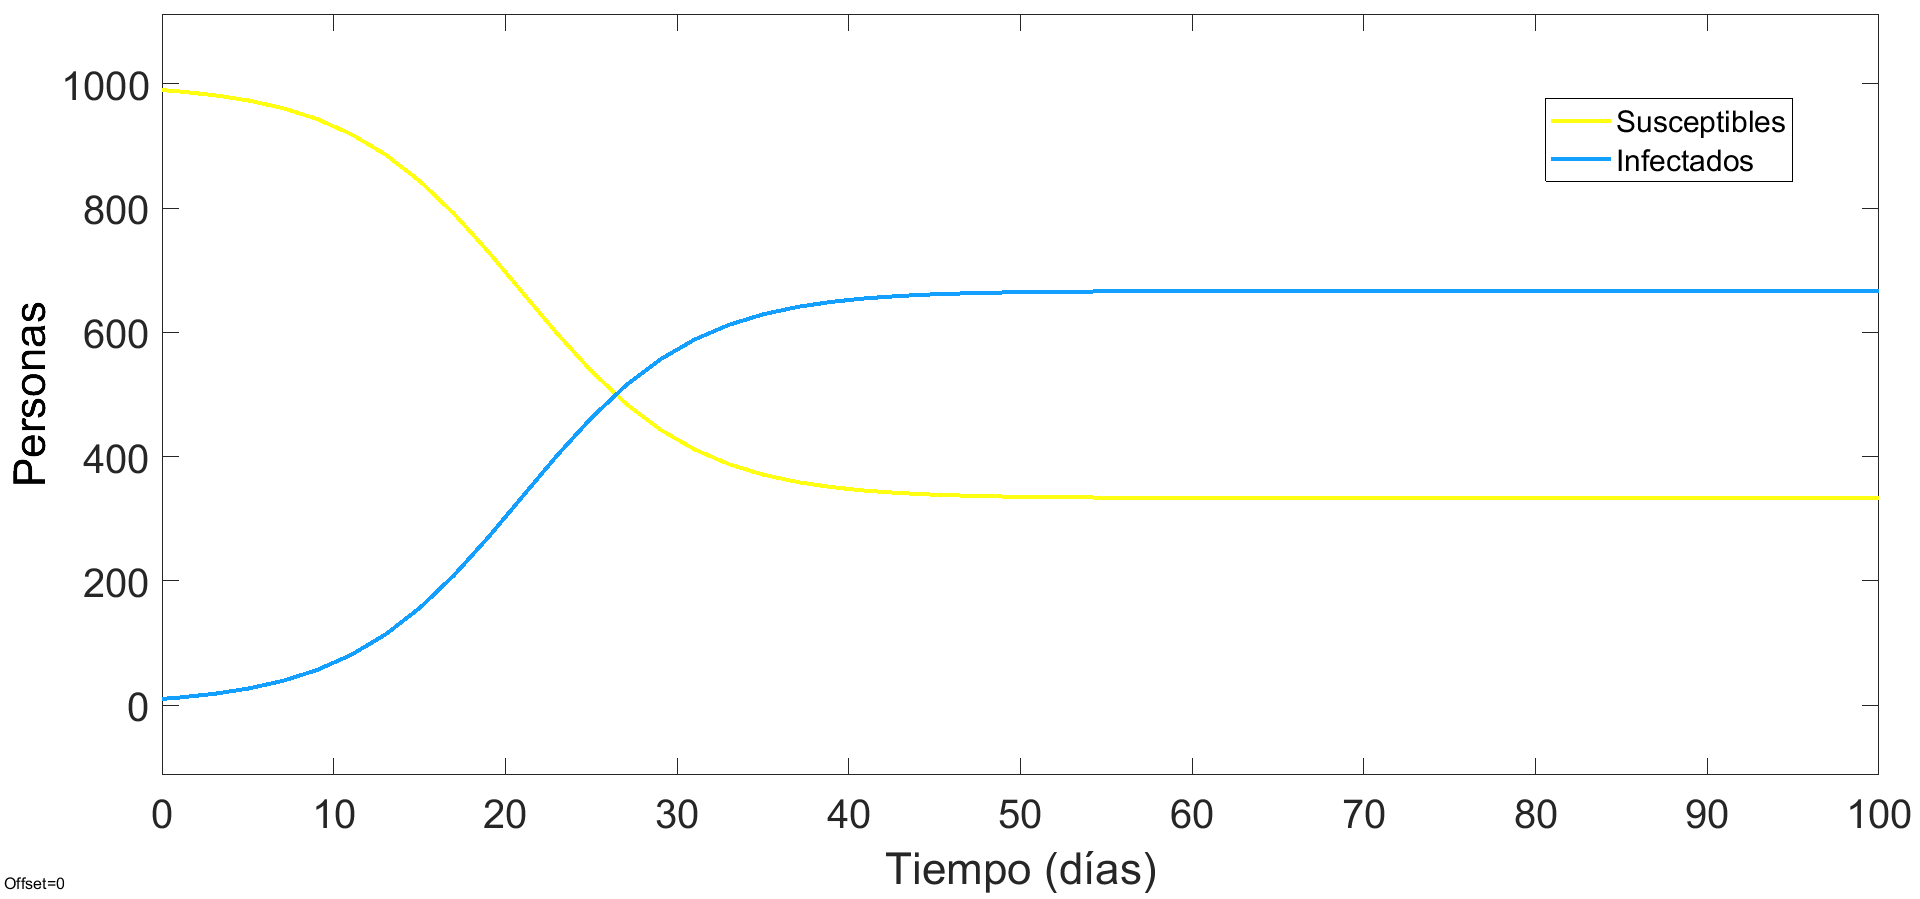
\includegraphics[width=0.7\textwidth]{img/modelo_SIS_resultado_ejemplo.png}
    \caption{Resultado típico de un modelo SIS.}
    \label{fig:ejeSIS}
    \vspace{0.5cm} % Ajusta el espacio vertical entre la imagen y el texto
\end{figure}


Rápido incremento en el número de individuos infectados, acompañado de una disminución pronunciada en la población susceptible. Este comportamiento inicial se debe a la alta tasa de transmisión.
Las curvas cambian sus pendientes: la velocidad de transmisión se compensa con la velocidad de recuperación, lo que da lugar a un punto de inflexión. El sistema tiende hacia un estado de equilibrio epidemiológico, donde los nuevos contagios son igual a las recuperaciones. Estabilización de ambas curvas.

Característica del modelo, en el cual los individuos se recuperan, pero no adquieren inmunidad, por lo que regresan al estado de susceptibles y pueden volver a infectarse. La enfermedad nunca desaparece completamente, sino que persiste en la población. Se alcanza así un equilibrio endémico.

Se calcula el número básico de reproducción como se ha explicado y para estos datos es $R_0$. Mayor que 1, la enfermedad se propaga y se mantiene en el tiempo. Este valor también explica el comportamiento observado en la gráfica (\ref{fig:ejeSIS}), crecimiento inicial de los casos seguido de una estabilización, lo que confirma que el borte ha alcanzado un equilibrio endémico estable.






\section{Modelo SIR}
El modelo SIR representa enfermedades donde los infectados se recuperan y adquieren inmunidad permanente. La población se divide en susceptibles, infectados y recuperados. Es útil para estudiar epidemias agudas y calcular el número básico de reproducción.

\textbf{Supuestos del modelo}. En este modelo se asume que la población total permanece constante, no hay nacimientos ni muertes. La inmunidad es permanente. Todos los individuos tienen la misma probabilidad de interactuar.
Aunque es un modelo idealizado, proporciona una herramienta para comprender y predecir el comportamiento de muchas enfermedades infecciosas, facilitando la toma de decisiones en salud pública y el diseño de estrategias de vacunación o contención.

Se muestra una representación esquemática del modelo SIS mediante el diagrama de flujo, representado en la figura \ref{fig:diagrama SIR}.
\begin{figure}[H]
    \centering
    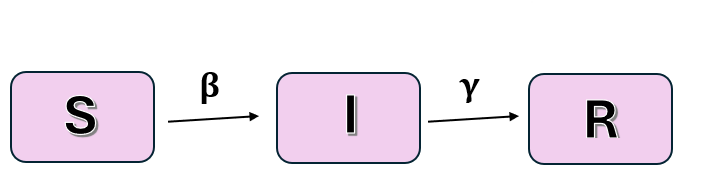
\includegraphics[width=0.7\textwidth]{img/diagrama_SIR.png}
    \caption{Diagrama de flujo modelo SIR.}
    \label{fig:diagrama SIR}
    \vspace{0.5cm} % Ajusta el espacio vertical entre la imagen y el texto
\end{figure}

También se puede representar el modelo mediante el siguiente sistema de ecuaciones diferenciales \eqref{eq:ec1SIR}\eqref{eq:ec2SIR}\eqref{eq:ec3SIR}.

\begin{align}
\frac{dS}{dt} &= -\beta SI \label{eq:ec1SIR} \\
\frac{dI}{dt} &= \beta SI - \gamma I \label{eq:ec2SIR} \\
\frac{dR}{dt} &= \gamma I \label{eq:ec3SIR}
\end{align}

Donde:
\begin{itemize}
    \item 	La ecuación dS⁄dt \eqref{eq:ec1SIR}, explica la disminución de individuos susceptibles debido a nuevos contagios. Depende del número de susceptibles, de infectados y de la tasa de contacto efectivo. El signo es negativo ya que los susceptibles disminuyen con el tiempo.
    \item 	La ecuación dI⁄dt \eqref{eq:ec2SIR}, refleja los dos procesos que afectan a los infectados, el aumento de los nuevos contagios y la disminución por las recuperaciones. La diferencia entre estos dos términos determina si el número de infectados crece o disminuye.
    \item 	La ecuación dR⁄dt \eqref{eq:ec3SIR}, describe como aumenta el número de recuperados. 
    \item El parámetro beta ($\beta$), tasa de transmisión o de contagio. Representa la probabilidad de que un contacto entre un individuo susceptible y uno infectado resulte en un nuevo contagio.
    \item 	El parámetro gamma ($\gamma$), tasa de recuperación. Probabilidad de que un individuo infectado se recupere y pase a recuperado.
\end{itemize}





El modelo se implementa en Simulink. Para mostrar su funcionamiento y lo que sería un resultado típico de este modelo, se realiza una simulación utilizando datos aleatorios, con el objetivo de observar el comportamiento del modelo SIR en un caso práctico, se oberva en la figura \ref{fig:ejemplo SIR}. La población total es de 10000, siendo susceptibles iniciales 9900 individuos, 100 individuos iniciales infectados y 0 individuos recuperados.
La tasa de transmisión es $\beta$ = 0,00003 y la tasa de recuperación es $\gamma$ 0.2



\begin{figure}[H]
    \centering
    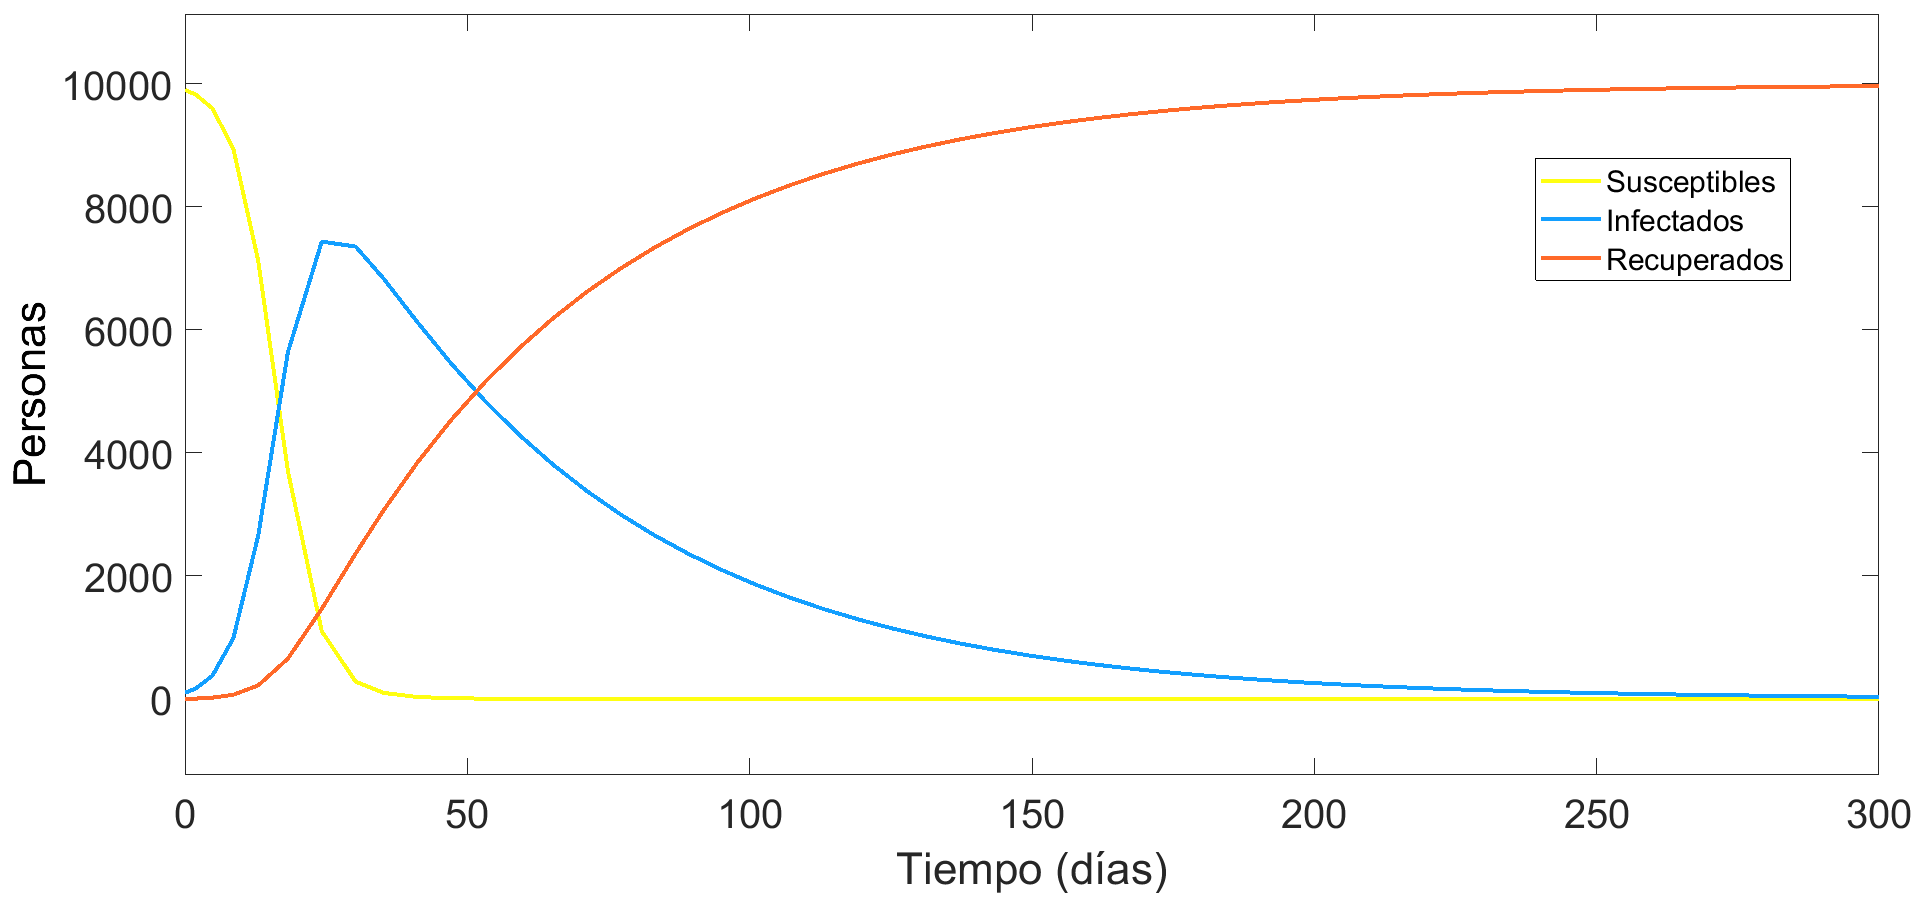
\includegraphics[width=0.7\textwidth]{img/modelo_SIR_resultado_ejemplo_.png}
    \caption{Resultado típico de un modelo SIR.}
    \label{fig:ejemplo SIR}
    \vspace{0.5cm} % Ajusta el espacio vertical entre la imagen y el texto
\end{figure}


En la gráfica \ref{fig:ejemplo SIR} se observa un comportamiento típico de una epidemia aguda.
Inicialmente, casi toda la población pertenece al compartimento de susceptibles. Desciende en los primeros días, debido a que una gran proporción de personas se infecta en un corto intervalo de tiempo. Esta rápida disminución refleja una enfermedad altamente contagiosa, que logra alcanzar a prácticamente toda la población susceptible.

El número de infectados crece de forma acelerada, alcanzando un máximo en el que se observa un gran número de personas enfermas a la vez. Sin embargo, a medida que estos infectados se recuperan y pasan al compartimento de recuperados, la curva de infectados comienza a descender.

La curva de recuperados comienza en cero y aumenta progresivamente, hasta que toda la población termina en este compartimento. Todos los individuos se recuperan de la enfermedad y adquieren inmunidad, lo que impide que la infección vuelva a propagarse. La inmunidad permanente es la que permite que la epidemia desaparezca de manera definitiva.

El número básico de reproducción con estos parámetros es $R_0$ = 15, indica que cada personas infectada contagia, de media a 15 individuos. La combinación de alta tasa de transmisión y tasa de recuperación relativamente baja favorece una propagación muy rápida, alcanzando una alta proporción de infectados al mismo tiempo. Esto lo se ve en el resultado de la figura \ref{fig:ejemplo SIR}.

Al ser un modelo SIR, los individuos que se recuperan no pueden volver a infectarse, a diferencia del modelo SIS, donde los recuperados vuelven al grupo de susceptibles. Esta diferencia es clave para entender por qué, en este caso, la epidemia se extingue completamente una vez que se alcanza la inmunidad de grupo, dejando a toda la población en el compartimento de recuperados.




\section{Modelo SEIR}
El modelo SEIR añade un estado de exposición al SIR, para representar enfermedades con periodo de incubación. Los individuos pasan de susceptibles a expuestos, luego a infectados y finalmente a recuperados con inmunidad. Relevante cuando se necesita considerar el impacto del periodo de incubación en la propagación de la enfermedad. Simplificación de la realidad, ofrece una aproximación más ajustada que el modelo SIR para muchas infecciones reales.

\textbf{Suposiciones del modelo}. En este modelo se asume también que la población total es constante, sin nacimientos ni muertes, y que los individuos solo atraviesan una vez cada uno de los estados. Asimismo, se supone una mezcla homogénea, es decir, todos los individuos tienen la misma probabilidad de interactuar entre sí.



Se muestra una representación esquemática del modelo SIS mediante el diagrama de flujo, representado en la figura \ref{fig:diagrama SEIR}.
\begin{figure}[H]
    \centering
    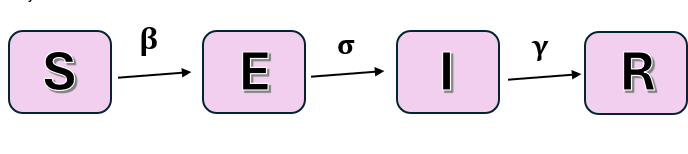
\includegraphics[width=0.7\textwidth]{img/diagrama_SEIR.png}
    \caption{Diagrma de flujo modelo SEIR.}
    \label{fig:diagrama SEIR}
    \vspace{0.5cm} % Ajusta el espacio vertical entre la imagen y el texto
\end{figure}

También se puede representar el modelo mediante el siguiente sistema de ecuaciones diferenciales \eqref{eq:dS_SEIR}\eqref{eq:dE_SEIR}\eqref{eq:dI_SEIR}\eqref{eq:dR_SEIR}. 
\begin{align}
\frac{dS}{dt} &= -\beta SI \label{eq:dS_SEIR} \\
\frac{dE}{dt} &= \beta SI - \sigma E \label{eq:dE_SEIR} \\
\frac{dI}{dt} &= \sigma E - \gamma I \label{eq:dI_SEIR} \\
\frac{dR}{dt} &= \gamma I \label{eq:dR_SEIR}
\end{align}

Donde:
\begin{itemize}
    \item 	La ecuación dS⁄dt \eqref{eq:dS_SEIR}, representa la disminución de individuos susceptibles por el contacto con personas infectadas. La disminución depende del número de susceptibles, del número de infectados y de la tasa de transmisión. Es negativa porque los susceptibles disminuyen con el tiempo al contagiarse.
    \item 	La ecuación dE⁄dt \eqref{eq:dE_SEIR}, describe el cambio en el número de individuos expuestos. Aumenta cuando un susceptible se infecta y disminuye cuando uno expuesto pasa a la fase infecciosa.
    \item 	La ecuación dI⁄dt \eqref{eq:dI_SEIR}, muestra la evolución de los infectados. Aumenta cuando los expuestos se vuelven contagiosos y disminuye por las recuperaciones. El balance entre estos dos procesos determina si el número de infectados crece o decrece.
    \item 	La ecuación dR⁄dt \eqref{eq:dR_SEIR}, refleja el aumento de individuos recuperados, que ya no pueden contagiarse ni contagiar. La velocidad de recuperación está determinada por la tasa de recuperación.
    \item Beta ($\beta$), tasa de transmisión: representa la probabilidad de que un individuo susceptible se infecte tras entrar en contacto con un infectado. 
    \item Sigma ($\sigma$), tasa de incubación: la inversa del tiempo medio que tarda un individuo expuesto en volverse contagioso. Se calcula como en la ecuación \eqref{eq:sigma1}.
    \begin{equation}
    \sigma = \frac{1}{\text{tiempo de incubación}}
    \label{eq:sigma1}
    \end{equation}
    \item Gamma ($\gamma$), tasa de recuperación: indica cuántos infectados se recuperan por unidad de tiempo. Es el inverso del tiempo medio de infección.
\end{itemize}

 

Es importante tener en cuenta la distinción entre individuos infectados e infecciosos, especialmente al comparar diferentes modelos epidemiológicos. En los modelos SIR y SIS se asume que un individuo infectado pasa inmediatamente a ser infeccioso, que puede transmitir la enfermedad en el mismo instante en que se contagia. 
Sin embargo, el modelo SEIR introduce una mejora al incorporar un compartimento de individuos \textbf{expuestos}. Cuando una persona susceptible entra en contacto con un individuo infeccioso, pasa primero al estado de \textbf{“expuesto”}, lo que significa que está infectada pero aún no es capaz de contagiar a otros. Este periodo representa el tiempo de incubación del patógeno, durante el cual el individuo no presenta síntomas y no es detectable clínicamente ni contagioso.
Tiene implicaciones relevantes al momento de establecer las condiciones iniciales para una simulación. 
En la práctica, no es posible conocer con exactitud cuántas personas se encuentran en el estado de exposición, ya que no presentan síntomas, no dan positivo en pruebas diagnósticas y tampoco tienen capacidad de contagiar.
Por esta razón, se va a asumir que el número inicial de expuestos es cero en las simulaciones. Aun así, este compartimento resulta fundamental para modelar de forma más realista enfermedades que incluyen un periodo de incubación significativo.


El modelo se implementa en Simulink. Para mostrar su funcionamiento y lo que sería un resultado típico de este modelo, se realiza una simulación utilizando datos aleatorios, con el objetivo de observar el comportamiento del modelo SEIR en un caso práctico \ref{fig:eje SEIR}. La población total es de 1000, siendo susceptibles iniciales 990 individuos, 10 individuos iniciales infectados y tanto expuestos como recuperados 0 individuos.
La tasa de transmisión es $\beta$ = 0,0005, la tasa de recuperación es $\gamma$ = 0,071 y la tasa de incubación es de $\sigma$ = 0,19 .

\begin{figure}[H]
    \centering
    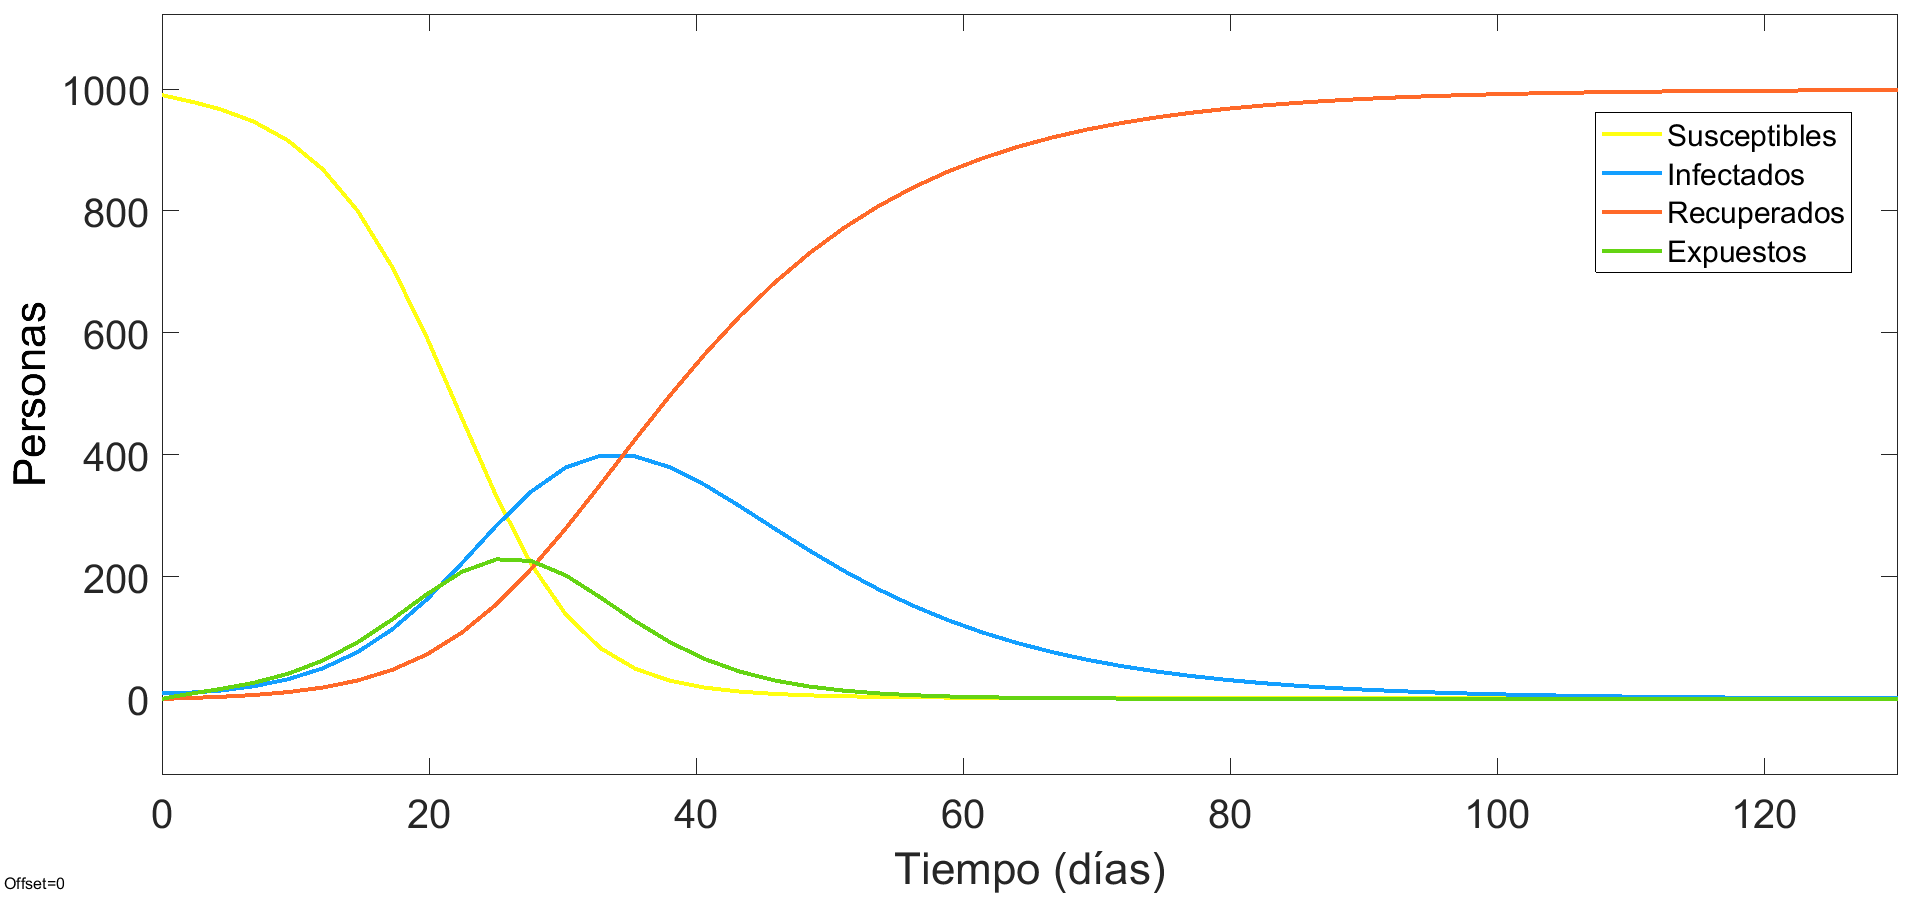
\includegraphics[width=0.7\textwidth]{img/modelo_SEIR_resultado_ejemplo.png}
    \caption{Resultado típico de un modelo SEIR.}
    \label{fig:eje SEIR}
    \vspace{0.5cm} % Ajusta el espacio vertical entre la imagen y el texto
\end{figure}

Como se observa en la figura \ref{fig:eje SEIR} al inicio, casi toda la población es susceptible, existe alto riesgo de contagio. A medida que los susceptibles se infectan pasan al compartimento de expuestos, lo que hace que el número de susceptibles disminuya rápido en las fases iniciales del brote.

El número de expuestos comienza siendo cero, pero crece rápido conforme se producen nuevos contagios. Estas personas están infectadas, pero no contagiosas debido al período de incubación. Por esta razón, la curva de los expuestos alcanza su pico antes que la de los infectados. 
La población infectada aumenta a medida que los expuestos se vuelven infecciosos. El número de infectados alcanza su máximo cuando el ritmo de nuevos contagios supera al de las recuperaciones. A medida que los infectados se recuperan, el número de personas en este compartimento comienza a descender.

Finalmente, el compartimento de recuperados incrementa a medida que los infectados superan la enfermedad y adquieren inmunidad permanente. Esta curva se estabiliza cuando la mayoría de la población ha pasado ya por la enfermedad, indicando el fin de la epidemia.
Importante calcular el número básico de reproducción con estos parámetros, $R_0$ es 7, con lo que es mayor que 1, por lo tanto la enfermedad tiende a crecer, se ve que en la gráfica \ref{fig:eje SEIR} se cumple este comportamiento.






\section{Medidas de control}

Se han incorporado dos medidas principales de control epidemiológico con el objetivo de reducir el impacto de la propagación de la enfermedad
\begin{itemize}
    \item \textbf{Vacunación preventiva}. Se ha añadido un término de vacunación a los modelos SIR y SEIR, permitiendo que la población susceptible adquiera inmunidad sin necesidad de haber pasado por la enfermedad. Esta estrategia representa una intervención sanitaria proactiva, donde una fracción de la población susceptible pasa directamente al compartimento de los inmunizados o recuperados. De este modo, se reduce la cantidad de personas expuestas al virus y, en consecuencia, el número total de infectados a lo largo del tiempo.
    \item \textbf{Control dinámico mediante regulador PID}. En el modelo SIR, se ha implementado un regulador PID que actúa sobre el parámetro $\beta$, correspondiente a la tasa de transmisión de la enfermedad. El objetivo del controlador es mantener el número de individuos infectados cercano a un valor de referencia o setpoint, evitando así un pico epidémico elevado que pueda sobrecargar el sistema sanitario.
   Este control simula políticas como cuarentenas, distanciamiento social, o uso de mascarillas, cuya intensidad se ajusta automáticamente en función de la evolución de los casos activos. Cuanto más se desvían los infectados del valor deseado, mayor es la intervención del regulador para reducir la transmisión, modificando $\beta$ en tiempo real.
\end{itemize}

\subsection{Mejora del modelo SIR}
Mejorar el modelo SIR como medida de control, incorporando explícitamente el efecto de la vacunación. Esta adaptación se conoce como modelo \textbf{SIRV} (Susceptibles – Infectados – Recuperados – Vacunados) y permite representar de forma más precisa la evolución de enfermedades infecciosas en poblaciones donde existen campañas de inmunización.

En el modelo SIRV, las personas susceptibles pueden infectarse al entrar en contacto con individuos contagiados, pero también tienen la opción de vacunarse como medida preventiva. Se asume que la vacunación confiere inmunidad completa y permanente, lo que implica que los individuos vacunados no pueden contraer la enfermedad ni transmitirla, y permanecen en ese estado de forma indefinida. De este modo, el grupo de vacunados actúa como una barrera adicional a la propagación del virus, reduciendo la proporción de personas susceptibles en la población y limitando la posibilidad de nuevos brotes.

Esta mejora del modelo permite analizar el impacto de diferentes tasas de vacunación sobre la evolución de la enfermedad y estudiar posibles estrategias de control. Además, ofrece una visión más ajustada a la situación actual, en la que la vacunación juega un papel fundamental en la protección individual y colectiva frente a enfermedades.

\textbf{Supuestos del modelo}. Es importante señalar que se mantienen los mismos supuestos básicos que en el modelo SIR. La única diferencia es la incorporación de la vacunación como medida de control de la enfermedad.

Se muestra una representación esquemática del modelo SIS mediante el diagrama de flujo, representado en la figura \ref{fig:ejemplo SIRV}.

\begin{figure}[H]
    \centering
    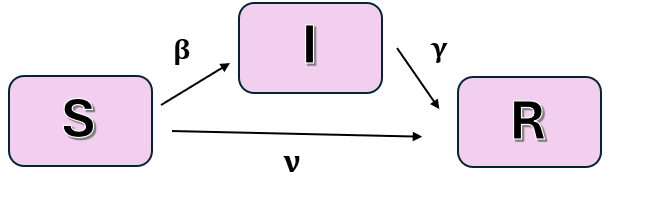
\includegraphics[width=0.7\textwidth]{img/diagrama_SIRV.png}
    \caption{Diagrma de flujo modelo SIRV.}
    \label{fig:ejemplo SIRV}
    \vspace{0.5cm} % Ajusta el espacio vertical entre la imagen y el texto
\end{figure}

También se puede representar el modelo mediante el siguiente sistema de ecuaciones diferenciales \eqref{eq:ec1SIRV}\eqref{eq:ec2SIRV}\eqref{eq:ec3SIRV}.
\begin{align}
\frac{dS}{dt} &= -\beta SI - \nu S \label{eq:ec1SIRV} \\
\frac{dI}{dt} &= \beta SI - \gamma I \label{eq:ec2SIRV} \\
\frac{dR}{dt} &= \gamma I + \nu S \label{eq:ec3SIRV}
\end{align}

Donde:
\begin{itemize}
    \item 	La ecuación ds⁄dt \eqref{eq:ec1SIRV}, representa la disminución del número de personas susceptibles con el tiempo. Se reduce el número por dos mecanismos contagio y vacunación. Cuando los susceptibles entran en contacto con infectados, se contagian y dejan de ser susceptibles. Cuando los susceptibles se vacunan, también abandonan este estado. El signo negativo indica que la población susceptible disminuye con el tiempo.
    \item 	La ecuación dI⁄dt \eqref{eq:ec2SIRV}, describe la evolución del número de infectados. Aumenta por nuevos contagios y disminuye por recuperación. La diferencia entre los dos términos determina si el número de infectados crece generando un brote epidémico o decrece produciéndose un control de la enfermedad.
    \item 	La ecuación dR⁄dt \eqref{eq:ec3SIRV}, muestra como aumenta el número de personas inmunizadas. Se incluyen tanto a las personas recuperadas de la enfermedad como a los vacunados que pasan directamente al estado inmune. El crecimiento del comportamiento recuperado refleja la inmunidad de la población.
    \item 	Beta ($\beta$): tasa de transmisión o contagio, ya explicada anteriormente.
    \item 	Gamma ($\gamma$): tasa de recuperación, explicada anteriormente.
    \item	Nu ($\nu$): tasa de vacunación. Nuevo parámetro incluido que va a representar la fracción de la población susceptible que se vacuna por unidad de tiempo. Permite estudiar distintos escenarios de intervención sanitaria mediante campañas de vacunación. Sus unidades son
\[
[\text{tiempo}]^{-1}
\]

Es importante señalar que, normalmente, lo que se encuentra en los datos disponibles es la \textbf{cobertura de vacunación}, entendida como la proporción de la población objetivo que ha sido vacunada. Sin embargo, para parametrizar modelos como el SIRV, se requiere la \textbf{tasa de vacunación} ($\nu$), es decir, la velocidad a la que se vacunan los individuos susceptibles.

Suponiendo que la vacunación actúa de forma continua y a una tasa constante sobre los susceptibles, se puede modelar la evolución del compartimento $S$ mediante la siguiente ecuación diferencial \eqref{ecudifer}:


\begin{equation}
\frac{dS}{dt} = -\nu S
\label{ecudifer}
\end{equation}

La solución a esta ecuación es una función exponencial \eqref{funcioex} decreciente:

\begin{equation}
S(t) = S(0) e^{-\nu t}
\label{funcioex}
\end{equation}

La \textbf{cobertura de vacunación} en el tiempo se define como la fracción de la población que ha sido vacunada respecto a la población susceptible inicial, es decir \eqref{cobert}:

\begin{equation}
\text{Cobertura}(t) = 1 - \frac{S(t)}{S(0)} = 1 - e^{-\nu t}
\label{cobert}
\end{equation}

Despejando la tasa de vacunación $\nu$, se obtiene:

\begin{equation}
\nu = \frac{-\ln(1 - \text{Cobertura})}{t}
\label{vacu}
\end{equation}

Esta fórmula \eqref{vacu} permite estimar una tasa de vacunación promedio constante, a partir del tiempo transcurrido y la cobertura alcanzada. Es útil para parametrizar modelos SIRV en contextos donde se dispone de datos agregados de vacunación.





\end{itemize}

En este modelo no se ha incluido un compartimento explícito para los vacunados, ya que se asume que la vacunación proporciona una inmunidad equivalente a la adquirida tras pasar la enfermedad. Por lo tanto, las personas vacunadas son incorporadas de manera directa al compartimento de recuperados, simplificando así el modelo sin perder su capacidad explicativa. 

Es importante señalar que la tasa de transmisión ($\beta$) no varía directamente como consecuencia de la vacunación, ya que se trata de un parámetro biológico y social que describe la probabilidad de contagio efectivo entre un individuo susceptible y uno infectado por unidad de tiempo. Esta tasa depende de factores como la contagiosidad del virus, el número medio de contactos diarios entre personas y las medidas de comportamiento social.
Por tanto, $\beta$ se mantiene constante en el modelo si no cambian estos factores. Lo que se ve afectado es el número de susceptibles. Al disminuir el tamaño del grupo susceptible mediante la inmunización, también se reduce la probabilidad de que se produzcan nuevos contagios, incluso si $\beta$ permanece constante. Aunque el virus mantenga su capacidad de contagio, al haber menos personas susceptibles, disminuye el número efectivo de nuevas infecciones.


\subsection{Control PID para modelo SIR}
Con el objetivo de limitar la cantidad de personas infectadas, se incorporó un mecanismo de control basado en un regulador PID. Este controlador actúa modificando el parámetro $\beta$, lo que equivale a simular la implementación de medidas como el distanciamiento social, el confinamiento o el uso de mascarillas. El propósito del controlador es mantener el número de infectados cerca de un valor deseado\footnote{Setpoint.}.

El sistema fue resuelto numéricamente mediante el método de Euler en MATLAB. Tanto las ecuaciones del modelo SIR como el regulador PID se programaron en código, lo que permitió ajustar fácilmente los parámetros del controlador y analizar su impacto en distintos escenarios.

Los parámetros del controlador PID utilizados:
\begin{itemize}
    \item $K_p$ = 0.01

    Término proporcional: reacciona al error actual entre el número de infectados y el setpoint.
    Un valor moderado como este permite responder al brote sin reacciones bruscas.
    \item $K_i$ = 0.001

    Término integral: tiene en cuenta la acumulación del error en el tiempo.
    Un valor bajo como este evita que el controlador se vuelva inestable por acumulaciones prolongadas.
    \item $K_d$ = 0.01

    Término derivativo: responde a la velocidad de cambio del error (si el brote está creciendo rápido).
Con este valor se suaviza la respuesta del sistema ante cambios bruscos.
\end{itemize}
Seleccionados mediante ajuste manual, buscando una respuesta estable del sistema que redujera el pico de infectados sin generar oscilaciones no realistas. Esta elección permite aplicar medidas graduales, representando un equilibrio entre reacción rápida y control suave del brote.

Además, el valor inicial del error fue error\_prev = 0 y la componente integral acumulada comenzó en error\_int = 0. El PID calcula en cada instante de tiempo una corrección sobre $\beta$, en función del error entre el número actual de infectados y el valor objetivo (setpoint), utilizando la expresión \eqref{eq:beta_PID}.
\begin{equation}
\beta(t) = \beta_0 - K_p \cdot e(t) - K_i \cdot \sum_{i=0}^{t} e(i) \cdot \Delta t - K_d \cdot \frac{e(t) - e(t - 1)}{\Delta t}
\label{eq:beta_PID}
\end{equation}
Donde $e(t) = I(t) - I_{\text{setpoint}}$ es el error en cada paso temporal. Esta corrección permite simular una intervención proporcional a la gravedad del brote en cada momento, activando medidas más o menos estrictas según sea necesario.

En la figura \ref{fig:simu3pid} se muestra un ejemplo de la introducción de un regulador en el modelo. Se puede observar que el pico de infectados no alcanza un valor muy elevado, ya que el número de personas infectadas se mantiene aproximadamente en torno al valor de referencia (setpoint). A medida que la epidemia avanza y disminuye la cantidad de personas susceptibles, el número de infectados tiende a cero.
\begin{figure}[H]
    \centering
    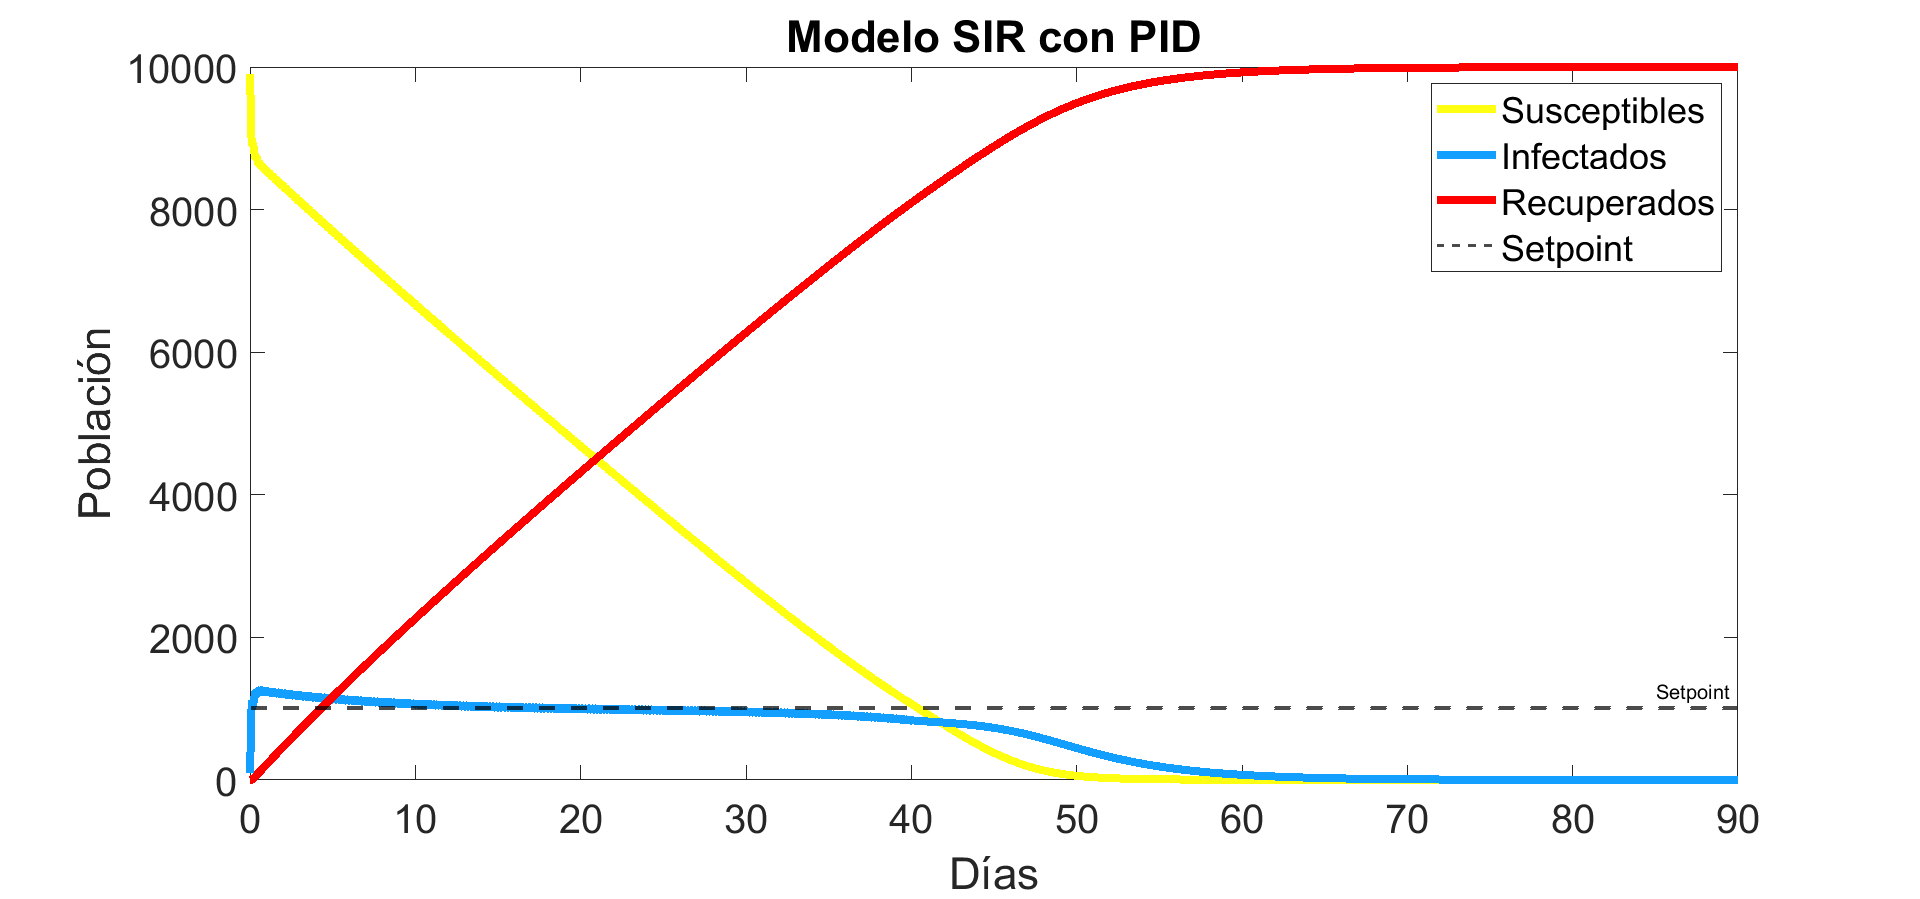
\includegraphics[width=0.7\textwidth]{img/modeloSIR_PID3.png}
    \caption{Simulación 1 para modelo SIR con PID.}
    \label{fig:simu3pid}
    \vspace{0.5cm} % Ajusta el espacio vertical entre la imagen y el texto
\end{figure}


\subsection{Mejora modelo SEIR}
Mejorar el modelo SEIR como medida de control, incorporando el explícitamente el efecto de la vacunación. Esta adaptación del modelo clásico SEIR se conoce como modelo \textbf{SEIRV} (Susceptibles – Expuestos – Infectados – Recuperados – Vacunados), se añaden los vacunados que representa a las personas que reciben una vacuna eficaz y desarrollan inmunidad contra el virus.

Se considera que las personas susceptibles pueden seguir el curso natural de exposición e infección o pasar directamente al grupo de inmunizados mediante vacunación, uniéndose al compartimento de recuperados, bajo el supuesto de que la inmunidad inducida por la vacuna es completa y duradera, al igual que en el caso de los individuos que se recuperan de la enfermedad. Aunque en la realidad la duración de la inmunidad puede variar y algunas vacunas no garantizan protección absoluta, esta simplificación permite estudiar de forma clara el efecto global de la inmunización sobre la propagación del virus.

Se muestra una representación esquemática del modelo SIS mediante el diagrama de flujo, representado en la figura \ref{fig:eje SEIRV}.

\begin{figure}[H]
    \centering
    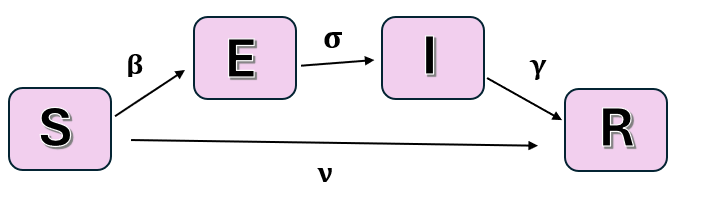
\includegraphics[width=0.7\textwidth]{img/diagrama_SEIRV.png}
    \caption{Diagrama de flujo del modelo SEIRV.}
    \label{fig:eje SEIRV}
    \vspace{0.5cm} % Ajusta el espacio vertical entre la imagen y el texto
\end{figure}
También se puede representar el modelo mediante el siguiente sistema de ecuaciones diferenciales \eqref{eq:dS_vacunacion}\eqref{eq:dE_SEIRV}\eqref{eq:dI_SEIRV}\eqref{eq:dR_vacunacion}.
\begin{align}
\frac{dS}{dt} &= -\beta SI - \nu S \label{eq:dS_vacunacion} \\
\frac{dE}{dt} &= \beta SI - \sigma E \label{eq:dE_SEIRV} \\
\frac{dI}{dt} &= \sigma E - \gamma I \label{eq:dI_SEIRV} \\
\frac{dR}{dt} &= \gamma I + \nu S \label{eq:dR_vacunacion}
\end{align}
Donde:
\begin{itemize}
    \item 	La ecuación dS⁄dt \eqref{eq:dS_vacunacion} representa la disminución de personas susceptibles con el tiempo. Este número disminuye por dos mecanismos el contagio y la vacunación. Por contagio cuando los susceptibles entran en contacto con infectados, se infectan y dejan de ser susceptibles. La vacunación los susceptibles salen del compartimento al ponerse la vacuna, ganando inmunidad directa sin tener que pasar por la enfermedad.
    \item 	La ecuación dE⁄dt \eqref{eq:dE_SEIRV} muestra el aumento de personas expuestas, personas infectadas que todavía no son contagiosas, debido a nuevos contagios, y su disminución a medida que pasan a estado de infectados. Aumentan por el término de contagio y disminuyen por el paso a infectados.
    \item 	La ecuación dI⁄dt \eqref{eq:dI_SEIRV}indica la variación del número de personas infectadas. Aumenta a medida que los expuestos se vuelven infecciosos y disminuye cuando los infectados se recuperan. Este balance determina su el número de infectados aumenta produciéndose una epidemia, o si por el contrario disminuye y se controla.
    \item La ecuación dR⁄dt \eqref{eq:dR_vacunacion}, muestra el aumento del número de personas inmunizadas. Se suman tanto los infectados que se recuperan como los susceptibles que se vacunan.
    \item 	Beta ($\beta$), tasa de transmisión: representa cuantos contagios ocurren por unidad de tiempo cuando una personas susceptible entra en contacto con una infectada.
    \item Sigma ($\sigma$), tasa de incubación. Inverso del tiempo de incubación.
    \item Gamma ($\sigma$), tasa de recuperación: inverso del tiempo de recuperación.
    \item 	Nu ($\nu$), tasa de vacunación: representa la fracción de la población susceptible que se vacuna por unidad de tiempo.
\end{itemize}

En este modelo no se ha incluido un compartimento explícito para los vacunados, ya que se asume que la vacunación proporciona una inmunidad equivalente a la adquirida tras pasar la enfermedad. Por lo tanto, las personas vacunadas son incorporadas de manera directa al compartimento de recuperados, simplificando el modelo sin perder su capacidad explicativa. Con la tasa de transmisión ocurre lo mismo a lo explicado para el modelo SIRV.




\section{Descripción de los datos}
Para cada uno de los modelos estudiados se ha seleccionado una enfermedad cuya dinámica se ajusta adecuadamente a la estructura del modelo. A continuación, se presentan los datos utilizados y se justifica la elección de cada enfermedad en función de las características del modelo correspondiente. Para más información ir a \textbf{Anexos, Apéndice D, apartado Datos utilizados.}

\subsection{Datos modelo SI}
El modelo SI es apropiado para representar enfermedades infecciosas crónicas como el VIH/SIDA, en las que una vez que una persona se infecta, permanece en ese estado de forma permanente. No contempla la recuperación, lo cual se ajusta al comportamiento del VIH, ya que, aunque existen tratamientos que permiten controlar la carga viral, no eliminan el virus del organismo.

En el modelo, la población se divide en dos grupos: S e I. Dado que el VIH no permite volver al estado susceptible ni alcanzar una recuperación definitiva, este enfoque resulta útil para analizar su propagación y estudiar la evolución de la enfermedad en función de parámetros clave como la tasa de transmisión ($\beta$).

\subsection{Datos modelo SIS}
La gonorrea es un ejemplo representativo de enfermedad que se ajusta al modelo SIS. En este modelo, los individuos pueden recuperarse, pero no adquieren inmunidad permanente, por lo que pueden reinfectarse. Esto refleja la dinámica de la gonorrea, ya que, tras el tratamiento, los pacientes pueden volver a contagiarse si se exponen de nuevo a la bacteria \textit{Neisseria gonorrhoeae}.
Este mecanismo de reinfección continua permite que la enfermedad persista en la población y alcance un equilibrio endémico. Por ello, el modelo SIS es una herramienta útil para estudiar su evolución y diseñar estrategias de control. 



\subsection{Datos modelo SIR}
El sarampión es una enfermedad vírica altamente contagiosa que se ajusta bien al modelo SIR. Este modelo describe enfermedades en las que los individuos, tras la recuperación, adquieren inmunidad permanente, como ocurre con el sarampión.
Presenta una transmisión muy eficiente, con un número básico de reproducción elevado, lo que facilita su propagación en poblaciones no inmunizadas. Además, tiene un periodo infeccioso definido, durante el cual puede transmitirse antes de que el individuo se recupere.

Históricamente, el sarampión causaba epidemias recurrentes, especialmente antes de la vacunación. Incluso hoy, cuando bajan las tasas de inmunización, pueden observarse rebrotes cuya dinámica encaja bien con las predicciones del modelo SIR. Por todo ello, el sarampión es un ejemplo claro de enfermedad modelable mediante este enfoque.



\vspace{2em}
\textbf{Modelo SIRV}. 





\subsection{Datos modelo SEIR}
El COVID-19 es una enfermedad que se ajusta bien al modelo SEIR, debido a la presencia de un periodo de incubación durante el cual los individuos están infectados pero aún no son contagiosos. Este periodo se representa mediante el compartimento de expuestos, característico de este modelo.

Tras la incubación, los individuos pasan a ser infectados, con o sin síntomas, y pueden transmitir el virus. Posteriormente, se recuperan y desarrollan cierta inmunidad, al menos temporalmente. Aunque esta inmunidad no siempre es permanente, el modelo SEIR básico permite representar de forma realista la dinámica de transmisión.
Gracias a esta correspondencia con las fases clínicas de la enfermedad, el modelo SEIR ha sido ampliamente utilizado para analizar la evolución del COVID-19, evaluar medidas de control y estimar la carga sanitaria en distintos escenarios.


\vspace{2em}


\textbf{Modelo SEIRV}. 






\section{Técnicas y herramientas}

\subsection{MATLAB}
\texttt{MATLAB} (acrónimo de MATrix LABoratory) \cite{mathworks_matlab} es una plataforma de programación y entorno de cálculo numérico desarrollada por MathWorks, diseñada para facilitar el análisis de datos, la creación de modelos matemáticos y el desarrollo de algoritmos. Gracias a su estructura basada en matrices y a su sintaxis intuitiva, permite realizar cálculos complejos y procesar grandes volúmenes de datos de forma eficiente. Su lenguaje de programación está optimizado para operaciones matemáticas, lo que lo hace más accesible que lenguajes tradicionales para tareas de análisis técnico.

El entorno incluye un completo IDE\footnote{Entorno de desarrollo integrado} que proporciona herramientas para la edición de código, visualización de datos, depuración y creación de interfaces gráficas. Además, cuenta con una amplia colección de toolboxes\footnote{Paquetes de herramientas adicionales} diseñados para áreas como el procesamiento de señales, control automático, aprendizaje automático o simulación de sistemas dinámicos.

\texttt{MATLAB} está disponible para los principales sistemas operativos. Su uso está extendido tanto en industria como en el ámbito académico, gracias a su versatilidad, documentación extensa y soporte técnico especializado. En entornos universitarios, su acceso suele estar facilitado mediante licencias institucionales, lo que permite a estudiantes y docentes utilizar todas sus funcionalidades sin coste adicional.

Aunque existen alternativas de código abierto , \texttt{MATLAB} se mantiene como una herramienta de referencia debido a su estabilidad, potencia en el tratamiento de datos numéricos y facilidad de uso, especialmente en tareas relacionadas con la ingeniería, las matemáticas aplicadas y las ciencias físicas.

\subsection{Simulink}
\texttt{Simulink} \cite{mathworks_simulink} es un entorno de simulación y diseño basado en diagramas de bloques, desarrollado por MathWorks e integrado de en \texttt{MATLAB}. Está orientado al modelado, simulación y análisis de sistemas dinámicos multidominio, que permite representar y estudiar el comportamiento de sistemas complejos mediante bloques funcionales interconectados. Gracias a su enfoque gráfico, \texttt{Simulink} facilita el desarrollo de modelos intuitivos y modulares sin necesidad de escribir código manual, aunque permite combinarlo con scripts de \texttt{MATLAB} para ampliar su funcionalidad.

\texttt{Simulink} se utiliza ampliamente en campos como el control automático, la electrónica, la ingeniería de comunicaciones, la automoción, la robótica, entre otros. Permite modelar sistemas en tiempo continuo, tiempo discreto o híbridos, incluyendo componentes físicos, señales lógicas, redes de control, sistemas mecánicos, eléctricos o térmicos. Su integración con toolboxes específicos amplía sus capacidades para abordar el modelado físico, la lógica de eventos o la optimización de controladores.

Una de las principales ventajas de \texttt{Simulink} es su capacidad de realizar una simulación previa a la implementación, permitiendo validar el comportamiento del sistema antes de llevarlo a hardware real. Además, ofrece herramientas avanzadas para el análisis de rendimiento, depuración de modelos, generación automática de código en C/C++ o HDL y conexión con sistemas de tiempo real.

En el ámbito académico, \texttt{Simulink} es una herramienta clave para enseñar conceptos de sistemas dinámicos, control y simulación, ya que su interfaz visual mejora la comprensión conceptual y reduce la curva de aprendizaje. Al igual que \texttt{MATLAB}, está disponible en muchas universidades mediante licencias académicas, lo que facilita su uso en proyectos de investigación, desarrollo y trabajos de fin de grado.

\subsection{App Desinger}
\texttt{App Designer} \cite{mathworks_matlab} es una herramienta integrada en \texttt{MATLAB} que permite crear aplicaciones interactivas con GUIs\footnote{Interfaces gráficas de usuario.} de forma visual e intuitiva. Está diseñada para facilitar el desarrollo de aplicaciones profesionales, combinando un entorno de diseño gráfico de componentes (botones, gráficos, deslizadores, tablas, etc.) con un editor de código basado en el lenguaje de \texttt{MATLAB}.

A diferencia de herramientas anteriores como \texttt{GUIDE}, \texttt{App Designer} ofrece una experiencia más moderna, con mayor integración, organización del código orientado a objetos, y funcionalidades avanzadas para el desarrollo de interfaces. Las aplicaciones creadas pueden ejecutarse directamente desde \texttt{MATLAB} o compartirse como aplicaciones independientes.

Esta herramienta es especialmente útil para prototipar algoritmos, visualizar datos de forma dinámica o crear herramientas personalizadas para usuarios finales, sin necesidad de conocimientos profundos en lenguajes de programación externos.

\subsection{LaTeX}
\texttt{LaTeX} \cite{latexproject} es un sistema de composición de textos de alta calidad, especialmente diseñado para la creación de documentos científicos y técnicos que requieren la presentación precisa de fórmulas matemáticas, gráficos y referencias bibliográficas. Debido a su potencia y flexibilidad, \texttt{LaTeX} es el estándar en la academia para la elaboración de informes, tesis y artículos científicos.

Para facilitar el trabajo colaborativo y la edición, se utilizó \texttt{Overleaf}, una plataforma en línea que permite editar, compilar y gestionar documentos \texttt{LaTeX} directamente desde el navegador web, sin necesidad de instalar software adicional. \texttt{Overleaf} también ofrece integración con sistemas de control de versiones y plantillas personalizadas, lo que mejora la organización y la eficiencia en la elaboración del documento.

\subsection{GitHub}
\texttt{GitHub} \cite{githubdocs} es una plataforma de desarrollo colaborativo que permite alojar, gestionar y controlar versiones de proyectos mediante el sistema de control de versiones \texttt{Git}. Su uso facilita el seguimiento del progreso del proyecto, el almacenamiento seguro del código y la colaboración entre múltiples desarrolladores.

En este proyecto, \texttt{GitHub} se ha utilizado como herramienta de control de versiones y respaldo del código fuente, incluyendo los modelos en \texttt{Simulink}, el desarrollo de la aplicación en \texttt{App Designer} y los documentos en \texttt{LaTeX}. Gracias a esta plataforma, ha sido posible mantener un historial detallado de los cambios realizados, identificar errores, volver a versiones anteriores del proyecto cuando ha sido necesario y garantizar una mayor organización y trazabilidad durante el desarrollo.

Además, al ser una plataforma en la nube, \texttt{GitHub} ha permitido trabajar desde diferentes dispositivos sin necesidad de configurar repositorios locales complejos, y ha servido como medio para compartir el proyecto en caso de ser necesario.


\capitulo{5}{Resultados}

\section{Comportamiento epidemia SIDA/VIH}

\section{Comportamiento epidemia gonorrea}

\section{Comportamiento epidemia sarampión}

\section{Comportamiento pandemia COVID-19}

\section{Discusión}


\capitulo{6}{Conclusiones}
Se ha llevado a cabo un estudio completo y detallado sobre el modelado determinista de epidemias, centrándose en los modelos clásicos SI, SIS, SIR y SEIR, que representan diferentes dinámicas de transmisión y recuperación de enfermedades infecciosas en una población. Se ha realizado una ampliación significativa en los modelos SIR y SEIR mediante la incorporación de la vacunación, bajo la hipótesis de que la inmunidad adquirida a través de la vacunación es equivalente a la obtenida tras la recuperación natural. Esta simplificación, aunque no considera variaciones en la eficacia de la vacuna o en la duración de la inmunidad, permite una aproximación adecuada para analizar el impacto de las estrategias de vacunación en la evolución de la epidemia.

Un aporte clave de este trabajo ha sido la implementación de un controlador PID en el modelo SIR, que simula medidas de intervención sanitaria como cuarentenas o restricciones sociales. La integración de este regulador posibilita un análisis más dinámico y realista, mostrando cómo la aplicación de políticas de control puede influir en la reducción de la transmisión y en el manejo de brotes epidémicos.

Para validar la utilidad y aplicabilidad de los modelos, se han empleado tanto datos aleatorios como datos reales. Los datos simulados han permitido examinar la respuesta teórica de los modelos bajo diferentes condiciones y parámetros, mientras que los datos reales han facilitado la comparación con situaciones epidémicas auténticas, evidenciando las fortalezas y limitaciones de cada modelo. Esto proporciona una visión práctica y fundamentada que puede ser de gran utilidad para profesionales en salud pública y modeladores matemáticos.

Además, se ha desarrollado una aplicación interactiva con una interfaz gráfica que hace posible visualizar de manera intuitiva y accesible el comportamiento de cada modelo. Esta herramienta está diseñada para que cualquier usuario, sin necesidad de conocimientos técnicos, pueda interactuar con los modelos y entender cómo distintas variables afectan la evolución de una epidemia. Esta accesibilidad contribuye a la difusión del conocimiento científico y puede apoyar la educación en temas de salud pública y prevención.


\section{Aspectos relevantes}
\begin{itemize}
    \item Estudio exhaustivo de modelos epidemiológicos deterministas, el análisis abarca cuatro modelos fundamentales en la epidemiología matemática: SI (susceptible-infectado), SIS (susceptible-infectado-susceptible), SIR (susceptible-infectado-recuperado) y SEIR (susceptible-expuesto-infectado-recuperado). Cada modelo representa distintas características y escenarios epidemiológicos, lo que permite comprender mejor cómo se propagan diferentes tipos de enfermedades infecciosas y las posibles transiciones entre estados.
    \item Incorporación de la vacunación en modelos SIR y SEIR. La introducción de la vacunación en estos modelos aporta un elemento crucial para el análisis de control epidémico, reflejando el efecto protector de las vacunas al desplazar individuos directamente al estado de inmunidad. Esto facilita la evaluación del impacto potencial de campañas de vacunación masiva, ayudando a predecir cómo puede cambiar la dinámica de contagios y la eventual reducción de la población susceptible.
    \item Diseño y aplicación de un regulador PID en el modelo SIR. El desarrollo de un controlador PID aplicado al modelo SIR representa un avance importante en la simulación de políticas públicas de control. Este controlador permite modelar intervenciones como cuarentenas, restricciones de movilidad y otras medidas no farmacológicas, evaluando su eficacia y optimizando su aplicación para mitigar el avance de la enfermedad.
    \item Uso combinado de datos aleatorios y datos reales para validación. El empleo de datos generados aleatoriamente ha sido esencial para probar la estabilidad y comportamiento de los modelos bajo diferentes escenarios hipotéticos. Por otro lado, la aplicación de datos reales permite una validación práctica, demostrando la capacidad predictiva de los modelos y su utilidad en la toma de decisiones en situaciones reales.
    \item Desarrollo de una aplicación gráfica accesible. La creación de una herramienta visual interactiva, amplía el alcance del trabajo al hacerlo accesible para un público más amplio, incluyendo profesionales, estudiantes y personas interesadas en el tema. La interfaz gráfica facilita la manipulación de parámetros y la observación de resultados en tiempo real, fomentando la comprensión y el aprendizaje de la dinámica epidémica.
    \item Relevancia para la salud pública y la educación. Más allá del aspecto técnico, el trabajo contribuye a la sensibilización y educación sobre la importancia del modelado matemático en la gestión de epidemias. Permite a usuarios no especializados comprender cómo diferentes factores afectan la propagación de enfermedades y la efectividad de intervenciones, apoyando así la difusión de información científica y la toma de decisiones informadas en contextos de salud pública.
    \item Posibilidad de futuras ampliaciones. El enfoque y las herramientas desarrolladas abren la puerta a futuras investigaciones, tales como la incorporación de modelos estocásticos, el análisis de inmunidad temporal, variantes virales, o la inclusión de factores sociales y económicos en la modelización, lo que puede enriquecer y actualizar las predicciones y estrategias de control epidémico.
\end{itemize}










\capitulo{7}{Líneas de trabajo futuras}


\bibliographystyle{apalike}
\bibliography{bibliografia}

\end{document}
